\documentclass{article}
\usepackage[a4paper,left=2cm,right=2cm,top=2cm,bottom=2.5cm]{geometry} 
\usepackage[utf8]{inputenc}
\usepackage[ngerman]{babel}
\usepackage{amsmath}
\usepackage[onehalfspacing]{setspace}
\usepackage{paralist}
\usepackage{graphicx}
\usepackage{epstopdf}
\usepackage[hidelinks]{hyperref}
\usepackage{caption}
\usepackage{subcaption}
\usepackage{amssymb}
\usepackage{pbox}

\setlength\parindent{0pt}
\setlength{\parskip}{8pt}
\renewcommand{\arraystretch}{1.5}

% Test -> paragraph wird quasi "subsubsubsection"
\usepackage{titlesec}

\setcounter{secnumdepth}{4}

\titleformat{\paragraph}
{\normalfont\normalsize\bfseries}{\theparagraph}{1em}{}
\titlespacing*{\paragraph}
{0pt}{3.25ex plus 1ex minus .2ex}{1.5ex plus .2ex}

% Test 2 -> subparagraph bekommt Umbruch

\titleformat{\subparagraph}
    {\normalfont\normalsize\bfseries\itshape}{\thesubparagraph}{1em}{}
\titlespacing*{\subparagraph}{\parindent}{3.25ex plus 1ex minus .2ex}{.75ex plus .1ex}

\numberwithin{equation}{section}

\begin{document}

\begin{center}

\thispagestyle{empty}

\vspace*{4cm}

\LARGE Zusammenfassung

\Huge Multivariate Verfahren

\Large in der Psychologie

\vspace*{8cm}

\large Carlo Michaelis

\large Wintersemester 2015/2016

\vspace*{0.3cm}

\normalsize Basierend auf einer Vorlesung

\normalsize von Prof. Dr. Manuel Völkle

\vfill

\normalsize{Dieses Dokument ist unter folgender Lizenz veröffentlicht:\\ \href{http://creativecommons.org/licenses/by-sa/4.0/}{Attribution-ShareAlike 4.0 International (CC BY-SA 4.0)}}


\end{center}

\newpage

\tableofcontents

\newpage

% #########################
% ##### 1. Einführung #####
% #########################

\section{Einführung}

\subsection{Psychologische Methodenlehre}

Eine \textbf{Theorie} ist ein System von Aussagen zur (1) Beschreibung, (2) Erklärung, (3) Vorhersage und der (4) Modifikation von (primär menschlichem) Erleben und Verhalten.

In der \textbf{psychologischen Methodenlehre} werden psychologische Theorien überprüft.

\subsubsection{Kriterien einer Theorie}

Eine Theorie muss folgende Kriterien erfüllen:

\begin{compactenum}
\item widerspruchsfrei
\item überprüfbar
\item explizit
\end{compactenum}

Dies führt zu einer \textbf{empirischen Verankerung}.

\subsection{Struktur eines Forschungsvorhabens \& Kriterien guter Forschung}

In jedem Schritt des Forschungsprozesses können Kriterien formuliert werden:

\begin{compactitem}
\item Problem
\item Sampling: Externe Validität
\item Design: Interne Validität
\item Messung: Konstruktvalidität
\item Analyse und Schlussfolgerung: Schlussfolgerungsvalidität
\end{compactitem}

Die Kriterien werden im Folgenden genauer betrachtet.

\subsubsection{Sampling}

In einer Messung werden folgende Größen erfasst:

\begin{compactitem}
\item Personen (Untersuchungseinheit)
\item Untersuchungsgegenstände (Variablen), z.B. Kognitive Fähigkeit
\item Situationen (Zeitpunkte)
\end{compactitem}

Diese werden gewöhnlich nicht in einer \textbf{Vollerhebung} bestimmt. Es wird nur eine \textbf{Stichprobe} betrachtet. D.h. nicht alle Personen, nicht alle Aspekte des Untersuchungsgegenstandes und nicht alle Situationen bzw. Zeitpunkte werden erfasst.

Ein Sampling kann in zwei Extremfällen erfolgen bzw. aus einer Mischform dieser Pole gewählt werden:

\begin{compactitem}
\item Zufalls-Sample (Random Sample)
\item Ausgewähltes Sample (Convenience Sample)
\end{compactitem}

Die \textbf{externe Validität} beschreibt den \emph{Grad der Generalisierbarkeit} über (1) Personen, (2) Situationen und (3) Untersuchungsgegenstände.

Der Sachverhalt kann in einem \textbf{Cattel'schen Datenquader} dargestellt werden.

In der \emph{multivariaten Forschung} werden Zusammenhänge zwischen mehreren abhängigen und unabhängigen Variablen betrachtet. Es werden mehrere Datenquader berücksichtigt.

\subsubsection{Untersuchungsdesign}

Wird nur eine Stichprobe betrachtet, können mögliche Drittvariablen einen Einfluss haben, die bei einem Sampling u.U. nicht erhoben wurden. Aussagen über Kausalität sind daher oft schwierige. Die \textbf{interne Validität} beschreibt den Grad in dem Aussagen über Ursache-Wirkungszusammenhänge möglich sind.

\subparagraph{Externe vs. interne Validität}

Um eine ideale interne Validität zu erhalten ist es nötig experimentelle Untersuchungen zu machen, bei denen möglichst viele Faktoren konstant gehalten werden. Dies führt meist jedoch zu einer geringeren externen Validität, da die Untersuchung damit konstruierter und weniger auf die Realität anwendbar ist, der Grad der Generalisierbarkeit ist geringer. Umgekehrt weisen Feld-Untersuchungen zwar einen hohe externe Validität auf, ihre Aussagekraft über Ursache-Wirkungszusammenhänge, und damit ihre interne Validität, ist jedoch eher gering.

\subsubsection*{Kausalität}

\subparagraph{Bedingungen für Kausalität}

Der Philosoph John Stuart Mill (1806-1873) formulierte drei Bedingungen für kausale Vorgänge:

\begin{compactenum}
\item Die Ursache muss dem Effekt zeitlich vorausgehen
\item Ursache und Effekt müssen zusammenhängen (kovariieren)
\item Alternative Erklärungsmöglichkeiten für den Ursache-Effekt-Zusammenhang müssen ausgeschlossen sein
\end{compactenum}

Problematisch ist aus methodischer Sicht vor allem die dritte Bedingung. Es ist sehr schwierig \emph{alle} alternativen Erklärungsmöglichkeiten auszuschließen.

\subparagraph{Definition der Kausalität}

Eine formelle Definition der Kausalität lieferte Paul Holland (1986). Dabei ergibt sich der \textbf{Kausaleffekt} durch:

\begin{equation}
\label{eq:causal-effect}
Y_{i|d=1} - Y_{i|d=0}
\end{equation}

Dabei bezeichnet $Y$ den Effekt $d=0$ bzw. $d=1$ jeweils an der Stelle $i$ (z.B. Personen, Zeitpunkt, etc.). Der Kausaleffekt könnte jedoch nur eindeutig erfasst werden, wenn die beiden subtrahierten Effekte an der gleichen Stelle $i$ erfasst werden. Werden sie nicht an der gleichen Stelle (z.B. gleiche Person, gleicher Zeitpunkt, etc.) erfasst, sollte davon ausgegangen werden, dass sich $Y$ bereits geändert hat. Holland formulierte \glqq \textbf{The Fundamental Problem of Causal Inference}\grqq.

\glqq It is impossible to observe the value of $Y_{i|d=1}$ and $Y_{i|d=0}$ on the same unit $i$ and, therefore, it is impossible to observe [but not infer] the effect on $i$.\grqq (Holland, 1986, p. 947).

Zur Lösung des Problems können zwei Ansätze gewählt werden:

\subparagraph{1. Ansatz, \glqq wissenschaftliche\grqq Lösung}

Bezüglich (1) Homogenität und (2) Invarianz werden Annahmen getroffen, die gemeinsam oder einzeln gültig sein müssen:

\begin{compactitem}
\item \emph{temporal stability} (Zeitliche Stabilität) und \emph{causal transience}
\item \emph{unit exchangeability}
\end{compactitem}

In Gleichung \ref{eq:causal-effect} bezeichne $i$ die Personen und die zusätzliche Variable $t$ die Zeit, dann kann z.B. davon ausgegangen werden, dass die Werte bei einer Messung $t$ genauso auch bei einer früheren Messung $t-1$ auftraten, sofern die gleichen Personen gemessen wurden. $Y_{i,t|d=0}$ ist somit äquivalent zu $Y_{i,t-1|d=0}$. Für de Kausaleffekt ergibt sich:

\begin{equation}
\gamma_i = Y_{i,t|d=1} - Y_{i,t-1|d=0}
\end{equation}

\subparagraph{2. Ansatz, Statistische Lösung}

Mittels des \emph{Erwartungswertes} werden durchschnittliche kausale Effekte betrachtet.

\begin{equation}
\gamma = \mathbb{E} \left[ Y_{i|d=1} - Y_{i|d=0} \right]
\end{equation}

Dabei können folgende Fälle verwendet werden:

\begin{compactenum}
\item \emph{Unterschiedliche Personen} $i$, $j$ zum \emph{gleichen Zeitpunkt} $t$: $E \left[ Y_{i,t=1|d=1} - Y_{j,t=1|d=0} \right]$
\item \emph{Gleiche Personen} $i$ zu \emph{unterschiedlichen Zeitpunkten} $t$: $E \left[ Y_{i,t=1|d=1} - Y_{i,t=0|d=0} \right]$
\item Kombinationen aus den ersten beiden Varianten.
\end{compactenum}

\subsubsection{Messung}
\label{sec:einf-messung}

Bei der Messung werden zwei Kriterien unterschieden:

\begin{compactitem}
\item \textbf{Reliabilität}: Güte der Messung
\item \textbf{Konstruktvalidität}: Güte des Konstrukts
\end{compactitem}

\subparagraph{1. Reliabilität}

Die Reliabilität ergibt sich über:

\begin{equation}
r_{tt} = \frac{\sigma^2_{wahr}}{\sigma^2_{gesamt}}
\end{equation}

Während die Gesamtvarianz $\sigma^2_{gesamt}$ bekannt ist, muss die wahre Varianz $\sigma^2_{wahr}$ geschätzt werden. Um einen Schätzer zu bestimmen werden folgende Axiome verwendet:

\begin{compactenum}
\item $X = T + \epsilon$ (Der gemessene Wert entspricht dem wahren Wert und dem Fehler)
\item $E[\epsilon] = 0$ (Im Mittel verschwindet der Fehler)
\item $Cov(T, \epsilon) = Cov(\epsilon_i, \epsilon_j) = 0$ (Der wahre Wert und der Fehler, sowie die Fehler untereinander sind unabhängig voneinander)
\end{compactenum}

Mit Hilfe der Axiome kann der wahre Wert geschätzt werden:

\begin{equation}
\sigma^2_{wahr} = Cov(X_A,X_B) \overset{(1)}{=} Cov(T+\epsilon_A,T+\epsilon_B) \overset{(3)}{=} Cov(T,T) + 0 + 0 + 0
\end{equation}

Die \textbf{Reliabilität} ist der Anteil der wahren Varianz an der Gesamtvarianz. Er bildet eine notwendige (nicht hinreichende) Voraussetzung für Korrelationen.

Die maximal mögliche Korrelation zwischen zwei Variablen $x$ und $y$ wird durch die Reliabilität begrenzt. Dies wird als \textbf{Attenuationskorrektur} bezeichnet:

\begin{equation}
\label{eq:korr-rel}
r_{wahr}(x,y) = \frac{r_{beob}(x,y)}{\sqrt{r_{tt}(x) \cdot r_{tt}(y)}}
\end{equation}

\subparagraph{2. Konstruktvalidität}

Selbst wenn die Messung \glqq technisch\grqq\ korrekt abläuft, kann es sein, dass das gewählte Konstrukt mit den gewählten Mitteln nicht vollständig erfasst wird. Vor allem wenn --- wie in der Psychologie häufig --- latente Konstrukte gemessen werden, ist es wichtig abschätzen zu können wie gut das jeweilige Konstrukt erfasst wird und nicht etwa ganz andere Konstrukte gemessen werden.

Egon Brunswik (1903-1955) beschäftigte sich mit der Frage, wie eine Messung konstruiert werden sollte, um sie valide zu gestalten. Ein zentraler Begriff ist dabei die \textbf{Symmetrie}. Wird bspw. der Einfluss des latenten Konstruktes \glqq Kognitive Fähigkeit\grqq\ auf den \glqq Durchschnitt der Schulnote\grqq\ betrachtet, müssen die gemessenen Aspekte der Konstrukte zueinander passen. Wird beispielsweise zur Erfassung der kognitiven Fähigkeit ein Test zur numerischen Verarbeitung durchgeführt und für die durchschnittliche Schulnote nur die Note im Fach Deutsch verwendet, so werden die Korrelationen gering ausfallen. Vielmehr sollte die verbale Fähigkeit erfasst werden oder alternativ nur die Note im Fach Mathe verwendet werden. Werden alle Fächer für die Durchschnittsnote berücksichtigt, so sollte auch die kognitive Fähigkeit möglichst umfassende Tests enthalten, um vernünftige Zusammenhänge zu erhalten. Da das Prinzip von Brunswik in Form einer Linse dargestellt werden kann, wird das Modell auch als \textbf{Linsenmodell} bezeichnet.

Die \textbf{Konstruktvalidität} beschreibt den Grad der Übereinstimmung von theoretischem und empirischen Konstrukt.

Auch die Konstruktvalidität begrenzt die maximale Korrelation zweiter Variablen. Gleichung \ref{eq:korr-rel} kann noch um den Einfluss der Konstruktvalidität $R(x)$, $R(y)$ und unbekannte Effekte $e$ (z.B. nonlineare Effekte, Selektionseffekte, etc.) ergänzt werden:

\begin{equation}
r_{wahr}(x,y) = \frac{r_{beob}(x,y)}{\sqrt{r_{tt}(x) \cdot r_{tt}(y)} \cdot R(x) \cdot R(y)} + e
\end{equation}

Effekte werden wegen mangelnder Validität häufig überschätzt.

\subsubsection{Analyse und Schlussfolgerung}

Im letzten Schritt, der Analyse und der Schlussfolgerung, welche im Folgenden genauer betrachtet werden, ist die \textbf{Schlussfolgerungsvalidität} ein letztes Kriterium. Sie beschreibt die Gültigkeit mit der inhaltliche
Schlussfolgerungen aus empirischen Daten gezogen werden.

\subsubsection*{Begriffe}

\fbox{\begin{minipage}{\textwidth}
Theorie, Psychologische Methodenlehre, Kriterien einer Theorie, Kriterien guter Forschung, Sampling, Vollerhebung, Stichprobe, Random Sample, Convenience Sample, externe Validität, Cattel'sches Datenquader, multivariate Forschung, Untersuchungsdesign, interne Validität, Zusammenhang interne/externe Validität, Bedingungen für Kausalität, Definition der Kausalität, Fundamental Problem of Causal Inference, Wissenschaftliche Lösung, Statistische Lösung, Reliabilität, Attenuationskorrektur, Konstruktvalidität, Linsenmodell, Schlussfolgerungsvalidität
\end{minipage}}

% ##########################################
% ##### 2. Multiple lineare Regression #####
% ##########################################

\section{Multiple lineare Regression}

\subsection{Grundlagen}
\label{sec:grund-reg}

\subsubsection{Komponenten der Regressionsgleichung}
\label{sec:komp-reg}

Es werden ausschließlich lineare Regressionsleichungen betrachtet, die Regressionskoeffizienten liegen in erster Potenz vor.

Popluationsregressionsfunktion mit der abhängien Variable $y$, den unabhängigen Variablen $x_k$ und den \textbf{Regressionskoeffizienten} bzw. \textbf{Regressionsgewichten} $b_k$ insbesondere der \textbf{Regressionskonstante} $b_0$ (y-Achsenabschnitt der Regressionsgeraden). $e$ ist der Fehler.

\begin{equation}
y = b_0 + b_1 x_1 + \dots + b_k x_k + \dots + b_n x_n + e
\label{eq:lin-regression}
\end{equation}

Bei der Stichprobenregressionsfunktion werden die Populationsparameter geschätzte:

\begin{equation}
y = \hat y + \hat e = \hat b_0 + \hat b_1 x_1 + \dots + \hat b_k x_k + \dots + \hat b_n x_n + \hat e
\end{equation}

Die Regresionskoeffizienten $b_k$ werden so geschätzt, dass die Summe der quadrierten Differenzen $\hat e$ zwischen vorhergesagten und beobachteten Werten $\hat y_i$ und $y_i$ über alle Personen $N$ minimal wird. Dies wird als \textbf{Methode der kleinsten Quadrate} bezeichnet.

\begin{equation}
\underset{\hat b_0, \dots, \hat b_n}{arg\,min} \left[ \sum_{i=1}^N (y_i - \hat y_i)^2 \right] = \underset{\hat b_0, \dots, \hat b_n}{arg\,min} \left[ \sum_{i=1}^N (\hat e_i)^2 \right] = \underset{\hat b_0, \dots, \hat b_n}{arg\,min} \left[ \sum_{i=1}^N (y_i - (\hat b_0 + \hat b_1 x_{1,i} + \dots + \hat b_k x_{k,i}))^2 \right]
\end{equation}

Für den Spezialfall eines Prädiktors (einer unabhängigen Variable) vereinfacht sich die Gleichung zu:

\begin{equation}
\label{eq:lineares-modell-2prae}
\underset{\hat b_0, \hat b_1}{arg\,min} \left[ \sum_{i=1}^N (y_i - \hat y_i)^2 \right] = \underset{\hat b_0, \hat b_1}{arg\,min} \left[ \sum_{i=1}^N (y_i - (\hat b_0 + \hat b_1 x_{1,i}))^2 \right]
\end{equation}

\begin{figure}
  \centering
  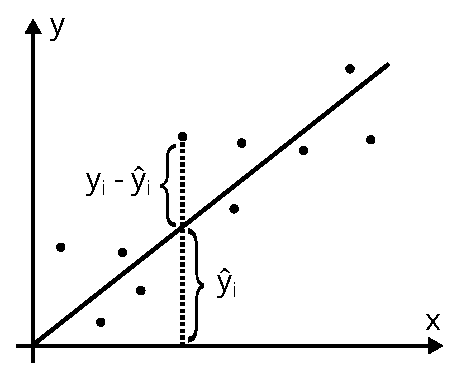
\includegraphics[width=0.4\textwidth]{images/lin-reg.eps}
  \caption{Lineare Regression. Mit den echten Werten $y_i$ und den geschätzten Werten $\hat y_i$.}
  \label{img:lin-reg}
\end{figure}

Ein anschauliches Beispiel ist in Abbildung \ref{img:lin-reg} dargestellt. Für 2 Prädiktoren ergibt sich eine Ebene, für 3 oder mehr Prädiktoren sind grafische Darstellungen nicht mehr anschaulich.

Anmerkung: Für die $x_k$ werden die Begriffe unabhängige Variable \& Prädiktor, für $y$ die Begriffe abhängige Variable \& Kriterium im Folgenden synonym verwendet.

\subsubsection{Partialregressionsgewichte}

Bei einer multiple Regression werden \textbf{partielle Regressionsgewichte} verwendet. Die Regressionsgewichte werden im Kontext der anderen Regressionsgewichte berechnet. Im Index wird dies deutlich gemacht, indem der erste Teil des Index den Index des betrachteten Koeffizienten ist, während der zweite Teil des Index den Indizes entsprechen, welche gerade nicht betrachtet werden. Während der Koeffizient eines Prädiktors variiert wird, werden die anderen Prädiktoren konstant gehalten.

\begin{equation}
\hat y_i = \hat b_{y0.1 \dots k \dots K} + \hat b_{y1.2 \dots k \dots K} x_{1,i} + \dots + \hat b_{yK.1 \dots k \dots K-1} x_{K,i}
\end{equation}

\subparagraph{Beispieldaten}

Die Fragestellung der Beispieldaten soll lauten:\\
Wie viel Dollar Gehalt verdient ein Professor abhängig von der Anzahl der Jahre im Beruf, der Anzahl der Publikationen, dem Geschlecht und der Anzahl der Zitationen?

Die Regressionskonstante (Intercept) gibt die Höhe des Gehaltes an (unstandardisiert, also in Dollar), ohne Beachtung der anderen unabhängigen Variablen (unter der Annahme alle anderen Koeffizienten wären Null). Der Intercept bildet den Ausgangspunkt. Das Regressionsgewicht einer Variable erhöht den Wert des Gehaltes multipliziert mit der Höhe des jeweiligen Wertes. Z.B. wird vorhergesagt, dass ein Professor pro Jahr $857,01\,\$$ mehr oder z.B. pro Zitation $201,93\,\$$ mehr verdient.

\subsubsection{Methode der kleinsten Quadrate (OLS): Bivariate Regression}

Bei bivariater Regression wird zunächst der Fall betrachtet, bei dem ein Prädiktor verwendet wird. Dazu wird von der Minimierungsfunktion aus Gleichung \ref{eq:lineares-modell-2prae} ausgegangen. Zur Bestimmung des Minimums werden die partiellen Ableitungen nach den Regressionsgewichten gebildet und Null gesetzt.

\begin{equation}
\frac{\partial}{\partial \hat b_0} \left[ \sum_{i=1}^N (y_i - (\hat b_0 + \hat b_1 x_{1,i}))^2 \right]  = 2 \cdot \left[ \sum_{i=1}^N y_i - (\hat b_0 + \hat b_1 x_{1,i}) \right] \cdot (-1) \overset{!}{=} 0
\end{equation}

\begin{equation}
\frac{\partial}{\partial \hat b_1} \left[ \sum_{i=1}^N (y_i - (\hat b_0 + \hat b_1 x_{1,i}))^2 \right] = 2 \cdot \left[ \sum_{i=1}^N y_i - (\hat b_0 + \hat b_1 x_{1,i}) \right] \cdot (-x_{1,i}) \overset{!}{=} 0
\end{equation}

Anschließend werden aus den zwei erhaltenen Gleichungen die Regressionsgewichte bestimmt.

\begin{equation}
\hat b_1 = \frac{N \sum_{i=1}^N (x_i \cdot y_i) - \sum_{i=1}^N x_i \cdot \sum_{i=1}^N y_i}{N \sum_{i=1}^N x_i^2 - (\sum_{i=1}^N x_i)^2}
\end{equation}

\begin{equation}
\hat b_0 = \frac{1}{N} \sum_{i=1}^{N} y_i - \hat b_1 \cdot \frac{1}{N} \sum{i=1}^N x_i
\end{equation}

\subsubsection{Methode der kleinsten Quadrate (OLS): Multiple Regression}

Im allgemeineren Fall werden $N$ Personen betrachtet. Das \textbf{Populationsregressionsmodell} kann in Matrixschreibweise wie folgt formuliert werden:

\begin{equation}
\mathbf{y} = \mathbf{X} \cdot \mathbf{b} + \mathbf{e}
\label{eq:lin-multi-regression}
\end{equation}

Ausgeschrieben entspricht dies für $K$ Prädiktoren und $N$ Personen:

\begin{equation}
\begin{pmatrix}
y_1\\ y_2\\ \vdots\\ y_N
\end{pmatrix}
=
\begin{pmatrix}
1 & x_{1,1} & \cdots & x_{1,K}\\
1 & x_{2,1} & \cdots & x_{2,K}\\
\vdots & \vdots & \ddots & \vdots\\
1 & x_{N,1} & \cdots & x_{N,K}\\
\end{pmatrix}
\begin{pmatrix}
b_0\\ b_1\\ \vdots\\ b_K
\end{pmatrix}
+
\begin{pmatrix}
e_1\\ e_2\\ \vdots\\ e_N
\end{pmatrix}
\end{equation}

Für das \textbf{Stichprobenregressionsmodell} gilt:

\begin{equation}
\label{eq:stichregmod}
\mathbf{y} = \mathbf{X} \cdot \mathbf{\hat b} + \mathbf{\hat e}
\end{equation}

Auch hier wird die Minimierungsfunktion so aufgestellt, dass der quadrierte Fehler $\hat e$ minimal wird:

\begin{equation}
\underset{\hat b_0, \dots, \hat b_n}{arg\,min} \left[ \sum_{i=1}^N (\hat e^i)^2 \right] = \underset{\hat b_0, \dots, \hat b_n}{arg\,min} \left( \mathbf{\hat e^T} \mathbf{\hat e} \right) \overset{(\ref{eq:stichregmod})}{=} \underset{\hat b_0, \dots, \hat b_n}{arg\,min} \left[ \left( \mathbf{y} - \mathbf{X}\mathbf{\hat b} \right)^T \left( \mathbf{y} - \mathbf{X}\mathbf{\hat b} \right) \right]
\end{equation}

Der innere Term wird als $SSE$ (\emph{Sum of Squared Errors}) bezeichnet. Nach Ausmultiplizieren kann dieser Term differenziert und Null gesetzt werden, um das Minimum zu bestimmen.

\begin{equation}
\begin{split}
\frac{\partial SSE}{\partial \mathbf{\hat b}} &= \frac{\partial }{\partial \mathbf{\hat b}} \left[ \left( \mathbf{y} - \mathbf{X}\mathbf{\hat b} \right)^T \left( \mathbf{y} - \mathbf{X}\mathbf{\hat b} \right) \right] \\
&= \frac{\partial }{\partial \mathbf{\hat b}} \left[ \mathbf{y^T y} - 2(\mathbf{y^T X \hat b}) + \mathbf{\hat b^T X^T X \hat b} \right] \\
&= -2 \mathbf{X^T y} + 2 \mathbf{X^T X \hat b} \overset{!}{=} 0
\end{split}
\end{equation}

Der Schätzer $\mathbf{\hat b}$ ergibt sich durch Umstellen der Gleichung:

\begin{equation}
\label{eq:schaetzer-b}
\mathbf{\hat b} = (\mathbf{X^T X})^{-1} \mathbf{X^T y}
\end{equation}

Durch einsetzen in das Stichprobenregressionsmodell in Gleichung \ref{eq:stichregmod} können Vorhersagen getroffen werden. Dabei entspricht $\mathbf{\hat y}$ der geschätzten Vorhersage. D.h. während $\mathbf{y} = \mathbf{X}\mathbf{\hat b} + \mathbf{\hat e}$ die gemessenen Daten beschreibt, beschreibt $\mathbf{\hat y} = \mathbf{X}\mathbf{\hat b}$ die vorhergesagten Daten. Für das Modell der geschätzten Werte gilt:

\begin{equation}
\mathbf{\hat y} = \mathbf{X}\mathbf{\hat b} \overset{(\ref{eq:schaetzer-b})}{=} \mathbf{X} (\mathbf{X^T X})^{-1} \mathbf{X^T y} = \mathbf{H y}
\end{equation}

Dabei beschreibt $\mathbf{H} = \mathbf{X} (\mathbf{X^T X})^{-1} \mathbf{X^T}$ den Zusammenhang zwischen den wahren Werten $\mathbf{y}$ und den geschätzten Werten $\mathbf{\hat y}$.

Die Diagonalelemente von $\mathbf{H}$ werde als \textbf{Leverage} bezeichnet. Der Leverage gibt an wie weit der Wert vom Mittel aller Prädiktoren $\mathbf{X}$ entfernt ist. Er bildet das \glqq Potential\grqq\ eines Wertes auf die Regressionsgerade Einfluss zu nehmen. Der Wert hat daher eine Art \glqq Hebelwirkung\grqq\ auf die Regression. Für einen einzelnen Prädiktor kann der Leverage wie folgt berechnet werden:

\begin{equation}
h_i = \frac{1}{N} + \frac{1}{N-1} \left( \frac{x_i - \bar x}{s_x} \right)^2
\end{equation}

\subsubsection{Standardisierte Regressionsgewichte}

Die \textbf{standardisierten Regressionsgewichte} werden durch \textbf{z-Standardisierung} aller Variablen vor der Regressionsanalyse erreicht. Für einen Prädiktor $\mathbf{X}$ gilt:

\begin{equation}
\mathbf{Z} = \frac{\mathbf{X}-\mu}{\sigma}
\end{equation}

Ist die Steigung eines Regressionsgewichtes beispielsweise $0.5$, so wird pro Erhöhung um ein entsprechendes $z$, die Ausgangsvariable um eine halbe Standardabweichung erhöht sein.

\subsubsection{Multiples R und Determinationskoeffizient}

Der Zusammenhang bzw. die Korrelation zwischen den beobachteten Werten $\mathbf{y}$ und den vorhergesagten Werten $\mathbf{\hat y}$ kann wie folgt berechnet werden.

\begin{equation}
R = Cor(y,\hat y) = \frac{Cov(y,\hat y)}{\sqrt{Var(y)\,Var(\hat y)}}
\end{equation}

Für zwei Prädiktoren entspricht die Korrelation der \emph{Pearson Produkt Moment Korrelation}. Im Fall mehrerer Prädiktoren wird die Korrelation als \textbf{multiples R} bezeichnet. Wird $R$ quadriert wird dies als \textbf{Determinationskoeffizient} (auch \textbf{Bestimmtheitsmaß}) $R^2$ bezeichnet. Er ist definiert mit der Variation von $\mathbf{y}$, die mit $SS_{total}$ (sum of squares) bezeichnet wird und der Variation der Residuen $SS_{residual}$:

\begin{equation}
\label{eq:determinationskoeff}
R^2 = 1 - \frac{SS_{residual}}{SS_{total}} = 1 - \frac{\sum_{i=1}^n (y_i - \hat y_i)^2}{\sum_{i=1}^n (y_i - \bar y_i)^2}
\end{equation}

Der Determinationskoeffizient ist somit ein Schätzer für die \emph{aufgeklärte Varianz}. Der Schätzer ist jedoch nicht \emph{erwartungstreu}, d.h. im Mittel entspricht der Koeffizient nicht der aufgeklärten Varianz in der Population $\rho^2$. Insbesondere bei kleinen Stichproben überschätzt $R^2$ auf Grund der Quadrierung die aufgeklärte wahre Varianz $\rho^2$. Zur Korrektur kann der \textbf{Adjusted} $\mathbf{R^2}$ (Korrigiertes $R^2$) verwendet werden, welcher den Anteil der aufgeklärten Varianz erwartungstreu angibt. Die Anzahl der Prädiktoren $K$ und der Stichprobenumfang (Anzahl der Personen) $N$ werden zur Korrektur verwendet.

\begin{equation}
\tilde{R}^2 = 1 - (1-R^2) \frac{N-1}{N-K-1}
\end{equation}

\subsubsection{Partial- und Semipartialkorrelation}

Die \textbf{quadrierte Semipartialkorrelation} gibt an wie stark der Prädiktor $k$ isoliert zur Gesamtvarianz beiträgt. Es gilt $k = 1,\dots,K$, wobei $K$ der Anzahl der Prädiktoren entspricht.

\begin{equation}
sr_k^2 = R^2_{1\dots k\dots K} - R^2_{1\dots k-1, k+1\dots K}
\end{equation}

Die \textbf{quadrierte Partialkorrelation} gibt an wie stark der Prädiktor $k$ isoliert zur Gesamtvarianz beiträgt, wobei der Wert ins Verhältnis zur unaufgeklärten Varianz (\textbf{Residualvarianz}) gesetzt wird. D.h. die Semipartialkorrelation wird durch die Varianz geteilt, die durch \emph{keine} Variable erklärt werden kann.

\begin{equation}
pr_k^2 = \frac{sr_k^2}{1 - R^2_{1\dots k-1, k+1\dots K}}
\end{equation}

Die Verhältnisse können in einem \textbf{Venn-Diagramm} (\emph{Ballantines}) veranschaulicht werden. Ein Beispiel ist in Abbildung \ref{img:venn} dargestellt. Die quadrierten Korrelationen können aus dem Venn-Diagramm anschaulich abgeleitet werden.

\begin{figure}
  \centering
  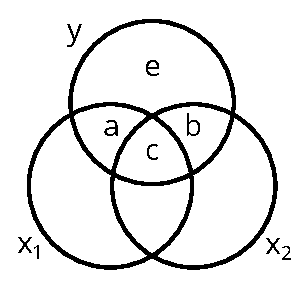
\includegraphics[width=0.3\textwidth]{images/venn.eps}
  \caption{Venn-Diagramm zur Veranschaulichung der Varianzanteile. $a$ entspricht der Varianz, die isoliert nur die Variable $x_1$ beiträgt. $b$ bezeichnet diejenige Varianz, die von $x_2$ aufgeklärt wird. $c$ wird von beiden Variablen $x_1$ und $x_2$ gemeinsam beigetragen. Der Anteil $e$ entspricht der Residualvarianz, die von keiner Variablen erklärt werden kann.}
  \label{img:venn}
\end{figure}

\begin{tabular}{llll}
$\bullet$ & Korrelation & $r^2_{y,x_1} = a + c$ & $r^2_{y,x_2} = b + c$\\
$\bullet$ & Semipartielle Korrelation & $sr^2_{y,x_1} = a$ & $sr^2_{y,x_2} = b$\\
$\bullet$ & Partielle Korrelation & $pr^2_{y,x_1} = \frac{a}{a+e}$ & $pr^2_{y,x_2} = \frac{b}{b+e}$\\
$\bullet$ & Multiple Korrelation & \multicolumn{2}{c}{$R^2_{y,x_1x_2} = a + b + c$}
\end{tabular}

\subsubsection{Statistische Inferenz}

Für die Parameterschätzer können Standardfehler berechnet werden. Sie geben die Güte des Schätzers an.

\subparagraph{Standardfehler der Regressionsgewichte}

\begin{equation}
SE_{b_k} = \frac{sd_y}{sd_k} \cdot \sqrt{\frac{1}{1-R_k^2}} \cdot \sqrt{\frac{1-R_y^2}{N-K-1}}
\end{equation}

Dabei wird $1-R_k^2$ als \textbf{Toleranz} bezeichnet. Sie beschreibt die unaufgeklärte Varianz der jeweiligen Variablen. $1-R_y^2$ wird als \textbf{Indeterminationskoeffizient} bezeichnet. Er bildet das Inverse des Determinationskoeffizienten $R_y^2$.

Der Standardfehler kann für verschiedene Verfahren verwendet werden:

1.) Das Regressionsgewicht $\hat b_k$ kann unter Annahme eines bestimmten Signifikanzniveaus $\alpha$ auf Signifikanz geprüft werden ($H_0: \, b_k = 0$). Der $t$-Wert für den \textbf{Hypothesentest} wird mit dem Standardfehler $SE_{b_k}$ bestimmt.

\begin{equation}
t_{1-\alpha,df} = \frac{\hat b_k}{SE_{b_k}} \quad \text{mit den Freiheitsgraden} \; df = N-K-1
\end{equation}

2.) Auf Basis des Standardfehlers kann das \textbf{Konfidenzintervall} bestimmt werden:

\begin{equation}
\label{eq:reggewicht-konfidenz}
C = \left[ \hat b_k - t_{1-\alpha,df} \cdot SE_{b_k} ; \, \hat b_k + t_{1-\alpha,df} \cdot SE_{b_k} \right]
\end{equation}

Wird das Niveau z.B. $\alpha = 0,05$ gewählt, dann wird mit der Gleichung \ref{eq:reggewicht-konfidenz} das $90\%$-Konfidenzintervall angegeben.

Die \emph{Interpretation des Konfidenzintervalls} ist streng genommen wie folgt: Werden mehrere Messungen durchgeführt und deren Konfidenzintervalle berechnet, so liegt der wahre Wert bei $90\%$ der bestimmten Konfidenzintervalle innerhalb des Intervalls. Die Annahme, der wahre Wert würde mit $90\%$-er Wahrscheinlichkeit innerhalb des Intervalls einer Messung liegen, ist nicht korrekt.

\subparagraph{Gesamt aufgeklärte Varianz und F-Test}
\label{sec:var-f-test}

Die gesamt aufgeklärte Varianz wird mittels des \textbf{F-Tests} auf Signifikanz geprüft. Die Nullhypothese lautet:

\begin{equation}
H_0: \, \rho^2 = 0 \quad \text{äquivalent zu} \quad H_0: \, b_1 = \dots = b_K = 0
\end{equation}

Die Prüfgröße (F-Wert) berechnet sich wie folgt:

\begin{equation}
F_{df_1,df_2} = \frac{R^2}{1-R^2} \frac{N-K-1}{K} \quad \text{mit} \; df_1 = K \;\text{(Zählerfr.)},\; df_2 = N-K-1 \;\text{(Nennerfr.)}
\end{equation}

Dabei ist $N$ die Größe der Stichprobe und $K$ die Anzahl der Prädiktoren.

Die Alternativhypothese $H_1$ lautet, dass mindestens ein $b_k \neq 0$ ist.

% #################################
% ##### Do it yourself Ansatz #####
% #################################

\subsubsection{Annahmen und Prüfung der multiplen linearen Regression (MLR)}
\label{sec:annahmen-alm}

Der multiplen linearen Regression (MLR) liegen \emph{5 Annahmen} zu Grunde.

\subparagraph{1. Linearität}

Der Zusammenhang zwischen unabhängigen und abhängigen Variablen muss linear sein. 

Dies bedeutet, dass die Regressionsterme linear additiv verknüpft sein müssen. Der Zusammenhang der Variablen muss jedoch \emph{nicht} linear sein. Erfüllt ist die Bedingung bspw. für:

\begin{compactitem}
\item $y = b_0 + b_1 x_1 + e $
\item $y = b_0 + b_1 \ln(x_1) + e$
\item $y = b_0 + b_1 x_1^2 + e$
\end{compactitem}

Zur anschaulichen Überprüfung eigenen sich \textbf{Residualplots} (x-Achse: Vorhergesagte Werte, y-Achse: Residuen). Der Verlauf muss hier ungefähr konstant bleiben.

\subparagraph{2. Exogene Prädiktoren}

Die Prädiktoren müssen perfekt reliabel sein, d.h. die Prädiktoren $\mathbf{X}$ müssen unabhängig vom Fehler $\mathbf{e}$ sein. Die Messung muss perfekt durchgeführt werden, damit die Messgrößen nicht von der Messung beeinflusst werden.

\begin{equation}
\mathbb{E}(e_i|\mathbf{X}) = 0
\end{equation}

Zur Überprüfung gibt es mehrere Möglichkeiten, z.B.:

\begin{compactitem}
\item Aufnahme weiterer Variablen ($\to$ Pfadanalyse, siehe Abschnitt~\ref{sec:pfadana})
\item Exogenität des Prädiktors durch Wahl des Versuchsdesigns
\item Reliabilität berechnen/kontrollieren
\end{compactitem}

Anmerkung: Die Berechnung der Korrelation zwischen $\mathbf{X}$ und $\mathbf{e}$ zur Überprüfung ergibt keinen Sinn. Per Annahme ist diese Korrelation Null.

\subparagraph{3. Homoskedastizität der Residuen}

Die Varianz der Residuen muss gleich sein, über den gesamten Bereich der vorhergesagten Werte. Mit anderen Worten: Die Varianz des $y$-Wertes an einer bestimmten Stelle muss mit den $y$-Werten an allen anderen Stellen übereinstimmen. Die Varianz entspricht dem \emph{quadrierten Standardschätzfehler}:

\begin{equation}
Var(\mathbf{\hat b}) = \mathbb{E} \left[ (\mathbf{X^T X})^{-1} \mathbf{X^T e e^T X} (\mathbf{X^T X})^-1 \right] = (\mathbf{X^T X})^{-1} \mathbf{X^T} \mathbb{E} [\mathbf{e e^T}] \mathbf{X} (\mathbf{X^T X})^-1
\end{equation}

Dabei ist $\mathbb{E} [\mathbf{e e^T}] = \sigma^2 \mathbf{1}$ die Homoskedastizitätsannahme.

Wie bei der 1. Annahme lässt sich auch diese gut mit Hilfe von \textbf{Residualplots} beurteilen. Die Varianz der Residuen sollte sich im Verlauf nicht ändern.

\subparagraph{4. Unabhängigkeit der Residuen}

Der Wert des Residuums eines Wertes, darf nicht von dem Wert des Residuums eines anderen Wertes abhängen. Es gilt, dass die einzelnen Werte \textbf{i.i.d.}, d.h. \glqq independent and identically distributed\grqq\ Verteilt sind.

Verletzt ist diese Annahme häufig bei (1) \emph{Clustering} oder (2) \emph{serieller Abhängigkeit}.

Ob eine Abhängigkeit vorliegt kann u.a. durch folgende Verfahren geprüft werden:

\begin{compactitem}
\item Theoretische Gründe (z.B. Schüler in einer Klasse, die Residuen werden über die Schüler mit der Klasse zusammenhängen)
\item Ausmaß des Clusterings (mittels Intraklassenkorrelation, hier nicht behandelt)
\item Ausmaß serieller Abhängigkeit (Prüfung z.B. durch Autokorrelation, $\to$ longitudinal data analysis)
\end{compactitem}

\subparagraph{5. Normalverteilung der Residuen}

Die Residuen sollten normalverteilt sein. Für große Stichproben ist die Annahme in der Praxis häufig nicht wichtig auf Grund asymptotischer Normalverteilung (\emph{Zentraler Grenzwertsatz}). Die Parameterschätzung bleibt unverzerrt. Problematisch ist es aber in (1) kleinen Stichproben. Außerdem indiziert eine fehlende Normalverteilung häufig (2) andere Probleme der Modellspezifikation.

Zur Überprüfung können z.B. (1) Histogramme oder (2) QQ-Plots eingesetzt werden.

Im Zweifelsfall, d.h. wenn es Probleme mit der Normalverteilungsannahme gibt (z.B. bei kleinen Stichproben), kann auf verteilungsfreie, d.h. nicht-parametrische Verfahren zurück gegriffen werden.

\subsubsection*{Begriffe}

\fbox{\begin{minipage}{\textwidth}
Komponenten der Regressionsgleichung, Methode der kleinsten Quadrate, Partielle Regressionsgewichte, Populationsregressionsmodell, Stichprobenregressionsmodell, SSE, Bivariate Regression, Multiple Regression, Leverage, z-Standardisierung, Standardisierte Regressionsgewichte, Determinationskoeffizient, Person-Produkt-Moment Korrelation, Multiples R, Adjusted $R^2$, Semipartialkorrelation, Bestimmtheitsmaß, Partialkorrelation, Residualvarianz, Venn-Diagramm, Standardfehler, Standardfehler Regressionsgewicht, Toleranz, Indeterminationskoeffizient, Hypothesentest, Konfidenzintervall, F-Test, Gesamt aufgeklärte Varianz, 5 Annahmen MLR, Linearität, Residualplots, Exogene Prädiktoren, Homoskedastizität, Quadrierter Standardschätzfehler, Unabhängigkeit Residuen, iid, Clustering, Serielle Abhängigkeit, Normalverteilung Residuen, QQ-Plots
\end{minipage}}

% ########################
% ##### Pfadanalyse ######
% ########################

\subsection{Pfadanalyse}
\label{sec:pfadana}

Mit der multiplen Regression können nicht nur Variablen vorhergesagt, sondern auch Hypothesen zum Zusammenhang von Variablen geprüft werden. Dies wird als \textbf{Pfadanalyse} bezeichnet. Auf Basis theoretischer Überlegungen werden \textbf{Kausalmodelle} (Causal Models) erstellt, welche die Zusammenhänge zwischen den Variablen angeben.

Der Kausalbegriff ist nur bedingt korrekt. Ein Kausalzusammenhang wird im Kontext einer Pfadanalyse so verstanden, dass ein kausaler Zusammenhang angenommen und entsprechend berechnet wird. Ob ein wirklicher kausaler Zusammenhang vorliegt, ist damit nicht gewährleistet.

Die Auswertung der Pfadanalyse erfolgt in zwei Schritten:

\begin{compactenum}
\item Zur Auswertung werden häufig \textbf{Pfaddiagramme} verwendet. Hiervon werden die \emph{Modellgleichungen} abgeleitet und die \emph{Pfadkoeffizienten} bzw. Regressionskoeffizienten bestimmt.
\item Das Modell wird an die Daten angepasst (\emph{Modellfit}). Je nach Ergebnis muss das Modell u.U. angepasst werden.
\end{compactenum}

Die Pfadanalyse kann als Vorläufer von Strukturgleichungsmodellen mit latenten Variablen verstanden werden, siehe Abschnitt \ref{sec:sem}. 

\subsubsection{Hierarchischer F-Test}

Der \textbf{hierarchische F-Test} bildet die Grundlage der Pfadanalyse. Der F-Test wurde (siehe Abschnitt \ref{sec:var-f-test}) eingesetzt um Varianzunterschiede zu testen. Der F-Test kann im Kontext der Pfadanalyse auch zur Testung von Unterschieden in \textbf{Sets} (Variablengruppen) verwendet werden. Die Prüfgröße (F-Wert) berechnet sich wie folgt:

\begin{equation}
F = \frac{R^2_{Y,AB} - R^2_{Y,A}}{1 - R^2_{Y,AB}} \cdot \frac{N-k_A-k_b-1}{k_B}
\end{equation}

Dabei ist $k_A$ die Anzahl der Variablen im Prädiktorset $A$, $k_B$ die Anzahl der Variablen im Prädiktorset $B$ und $N$ die Stichprobengröße. $R^2_{Y,AB}$ ist die multiple Korrelation mit den Sets $A$ und $B$, sie beschreibt wie gut $A$ und $B$ die Varianz von $Y$ erklären können. $R^2_{Y,A}$ ist die multiple Korrelation mit Set $A$, sie beschreibt wie gut $A$ die Varianz von $Y$ erklären kann. Der Zählerterm ${R^2_{Y,AB} - R^2_{Y,A}}$ beschreibt wie gut $B$ die Varianz von $Y$ erklären kann (aber auch unter Berücksichtigung von $A$), der Nennerterm ${1 - R^2_{Y,AB}}$ beschreibt den Anteil der Varianz, der durch $A$ und $B$ \emph{nicht} erklärt werden kann.

\subsubsection{Pfaddiagramme und Notation}

\begin{figure}[h]
  \centering
  \captionsetup{justification=centering}
  \begin{subfigure}[b]{0.3\textwidth}
    \centering
    
\includegraphics[width=0.3\textwidth]{images/pfad-symbole/manifest.png}
    \caption{Manifeste Variable\\ (beobachtet)}
  \end{subfigure}
  \begin{subfigure}[b]{0.3\textwidth}
    \centering
    
\includegraphics[width=0.3\textwidth]{images/pfad-symbole/latent.png}
    \caption{Latente Variable\\ (nicht beobachtet)}
  \end{subfigure}
  \begin{subfigure}[b]{0.3\textwidth}
    \centering
    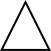
\includegraphics[width=0.3\textwidth]{images/pfad-symbole/konstant.png}
    \caption{Konstante\\ (Mittelwerte/Regress.)}
  \end{subfigure}
  \caption{Symbole für Variablen bei der Pfadanalyse. Latente Variablen werden auch als \glqq Faktoren\grqq\ oder \glqq Fehlerterme\grqq\ bezeichnet. Konstanten dienen zur Darstellung von Mittelwerten und Regressionskoeffizienten.}
  \label{img:pfad-symbole}
\end{figure}

\begin{figure}[h]
  \centering
  \captionsetup{justification=centering}
  \begin{subfigure}[b]{0.3\textwidth}
    \centering
    
\includegraphics[width=0.75\textwidth]{images/pfad-symbole/gerichtet.png}
    \caption{Gerichtete Beziehung\\ (\glqq Kausal\grqq -Pfad)}
  \end{subfigure}
  \begin{subfigure}[b]{0.3\textwidth}
    \centering
    
\includegraphics[width=0.75\textwidth]{images/pfad-symbole/ungerichtet.png}
    \caption{Ungerichtete Beziehung\\ (Kovarianz/Korrelation)}
  \end{subfigure}
  \begin{subfigure}[b]{0.3\textwidth}
    \centering
    
\includegraphics[width=0.75\textwidth]{images/pfad-symbole/reziprok.png}
    \caption{Reziproke/Feedback Beziehung\\ (Nicht-Rekursive Modelle)}
  \end{subfigure}
  \caption{Relationen zwischen Variablen bei der Pfadanalyse.}
  \label{img:pfad-relationen}
\end{figure}

Zur Erstellung von Pfaddiagrammen gibt es bestimmte Konventionen für die verwendeten Symbole. Die üblichen Symbole sind in Abbildung~\ref{img:pfad-symbole}, die Relationen in Abbildung \ref{img:pfad-relationen} dargestellt. Die grafische und mathematische Repräsentation ist häufig äquivalent. Oft dient sie jedoch auch der einfachen Illustration.

\textbf{Sprechweise}: \glqq Regression von $Y$ auf $X$\grqq\ entspricht der \glqq Vorhersage von $Y$ durch $X$\grqq

\subparagraph{Variablenarten}

\begin{compactitem}
\item \textbf{Manifeste/Latente Variablen}: Direkt beobachtete / nicht direkt beobachtete Variablen
\item \textbf{Endogene Variablen}: Variablen welche vorhergesagt werden (und nicht andere Variablen erklären)
\item \textbf{Exogene Variablen}: Variablen welche vorhersagen (und nicht durch andere erklärt werden)
\item \textbf{Mediatorvariablen}: Variablen welche Effekte vermitteln (von einer/mehrere Variablen auf eine/mehrere Variablen)
\item \textbf{Konfundierende Variablen}: Variablen welche in Wirklichkeit (zumindest teilweise) einen Effekt bewirken. Werden diese nicht berücksichtigt, kommt es zu Scheineffekten (siehe unten).
\item \textbf{Moderierende Variablen}: Variablen welche in Abhängigkeit zu einem Effekt stehen. Ändert sich die Variable, so ändert sich der Zusammenhang zwischen den ursprünglich betrachteten Variablen.
\item \textbf{Residualvariablen}: Latente Variablen welche die nicht-erklärte Varianz beschreiben
\end{compactitem}

Die Beziehungen einiger Variablenarten sind in Abbildung \ref{img:variablenarten} dargestellt.

\begin{figure}[h]
  \centering
  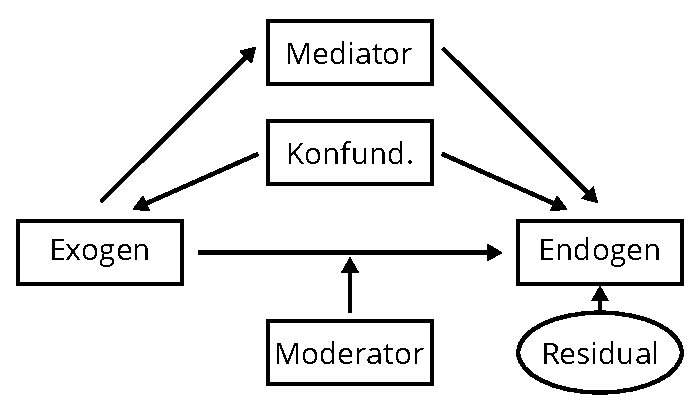
\includegraphics[width=0.5\textwidth]{images/variablenarten.eps}
  \caption{Variablenarten: Die Beziehung zwischen endogener und exogener Variabler mit Mediatorvariable, Moderatorvariable und konfundierender Variable, sowie einer latenten Residualvariable.}
  \label{img:variablenarten}
\end{figure}

\subparagraph{Effektarten}

\begin{compactitem}
\item \textbf{Direkter Effekt}: Effekt von einer Variablen auf eine andere Variable (unter Kontrolle aller anderen)
\item \textbf{Indirekter Effekt}: Effekt von einer Variablen auf eine andere Variable, über eine/mehrere andere Variablen (Mediatoreffekt)
\item \textbf{Totaler Effekt}: Summe aller indirekter Effekte addiert mit dem direkte Effekt einer Variablen
\item \textbf{Zero-Order-Effekt}: Effekt von einer Variablen auf eine andere Variable (unter Ignorierung aller anderen)
\item \textbf{Scheineffekt}: Differenz zwischen Zero-Order-Effekt und totalem Effekt
\end{compactitem}

Die Effekte sind in Abbildung~\ref{img:pfad-effekte} an Beispielen dargestellt.

\begin{figure}[h]
  \centering
  \captionsetup{justification=centering}
  \begin{subfigure}[b]{0.48\textwidth}
    \centering
    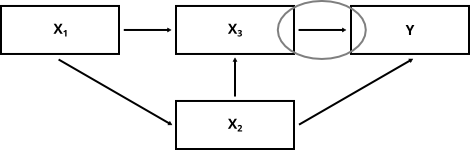
\includegraphics[width=0.85\textwidth]{images/pfad-effekte/direkt.png}
    \caption{Direkter Effekt von $X_3$ auf $Y$}
  \end{subfigure}
  \begin{subfigure}[b]{0.48\textwidth}
    \centering
    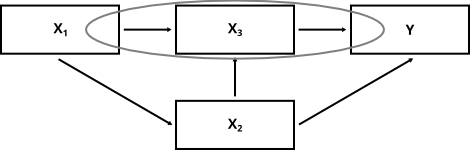
\includegraphics[width=0.85\textwidth]{images/pfad-effekte/indirekt.png}
    \caption{Indirekter Effekt von $X_1$ via $X_3$ auf $Y$}
  \end{subfigure}\vspace*{0.5cm}
  
  \begin{subfigure}[b]{0.48\textwidth}
    \centering
    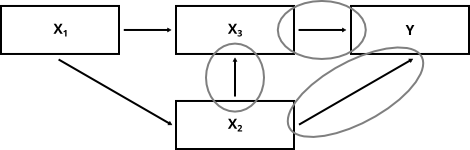
\includegraphics[width=0.85\textwidth]{images/pfad-effekte/total.png}
    \caption{Totaler Effekt von $X_2$ auf $Y$}
  \end{subfigure}
  \begin{subfigure}[b]{0.48\textwidth}
    \centering
    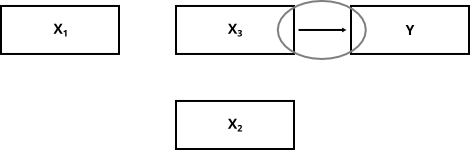
\includegraphics[width=0.85\textwidth]{images/pfad-effekte/zero-order.png}
    \caption{Zero-Order-Effekt von $X_3$ auf $Y$}
  \end{subfigure}
  \caption{Effekte zwischen Variablen bei der Pfadanalyse.}
  \label{img:pfad-effekte}
\end{figure}

\subparagraph{Rekursive/Nicht-Rekursive Pfadmodelle}

\textbf{Rekursive Pfadmodelle} erfüllen zwei Bedingungen:

\begin{compactenum}
\item Hierarchisch: Kausaler Fluss geht nur in eine Richtung
\item Wechselseitig unkorrelierte Residualterme (Residualterme hängen nicht miteinander zusammen)
\end{compactenum}

In der folgenden Betrachtung wird sich auf rekursive Pfadmodelle beschränkt. Zur Betrachtung nicht-rekursiver Modelle (z.B. mit Feedback-Schleifen) ist unter anderen Voraussetzung möglich.

Die Effekte in Pfadmodellen können im (1) \emph{hierarchischen} und im (2) \emph{simultanen} Ansatz bestimmt werden. Die Ansätze sollen anhand eines Beispiels betrachtet werden. Wieder wird das Beispiel von oben betrachtet. Es soll untersucht werden welche Faktoren das Gehalt eines Professors bestimmen. Das zu untersuchende Modell ist in Abbildung~\ref{img:pfad-hierarchisch} dargestellt.

\begin{figure}[h]
  \centering
  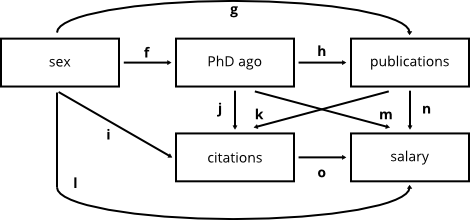
\includegraphics{images/pfad-hierarchisch.png}
  \caption{Beispiel-Modell der Einflüsse auf das Gehaltes eines Professors in der Pfadanalyse.}
  \label{img:pfad-hierarchisch}
\end{figure}

\subsubsection{Hierarchischer Ansatz}

Es sind viele verschiedene Einflüsse von Drittvariablen möglich. Um herauszufinden welche Drittvariablen eine Rolle spielen, wird im \textbf{hierarchischen Ansatz} ein Prädiktor nach dem anderen hinzugenommen (hierarchisch). Im Beispiel in Abbildung~\ref{img:pfad-hierarchisch} wäre das Vorgehen wie folgt:

\begin{compactenum}
\item sex $\to$ salary
\item sex \& PHD ago $\to$ salary
\item sex, PHD ago \& publications $\to$ salary
\item sex, PHD ago, publications \& citations $\to$ salary
\end{compactenum}

In dem Modell ergeben sich folgende Effekte:

\begin{compactitem}
\item Zero-Order-Effekt: $r_z = r_{sex,salary}$
\item Direkter Effekt: $r_d = r_l$
\item Indirekte Effekte: $r_c$ mit $c \in \{f,g,h,i,j,k,m,n,o\}$
  \begin{compactitem}
  \item via citations: $i \cdot o$
  \item via publications: $g \cdot n$ und $g \cdot k \cdot o$
  \item via PhD ago: $f \cdot m$, $f \cdot h \cdot n$, $f \cdot j \cdot o$ und $f \cdot h \cdot k \cdot o$
  \end{compactitem}
\item Totaler Effekt: $R = \sum r_{\text{indirekt}} + r_l = r_{io} + r_{gn} + r_{gko} + r_{fm} + r_{fhn} + r_{fjo} + r_{fhko} + r_l$
\end{compactitem}

Da überwiegend totale Effekte erfasst werden, erfolgt die Berechnung der indirekten Effekte durch Subtraktion.

\subsubsection{Simultaner Ansatz}

Im \textbf{simultanen Ansatz} wird die abhängige Variable variiert. In jedem Schritt wird eine unabhängige Variable mehr hinzugenommen, während gleichzeitig eine andere abhängige Variable gewählt wird. Es wird in der Reihenfolge des Modells vorgegangen. Im Beispiel in Abbildung~\ref{img:pfad-hierarchisch} wäre das Vorgehen wie folgt:

\begin{compactenum}
\item sex $\to$ PHD ago
\item sex \& PHD ago $\to$ publications
\item sex, PHD ago \& publications $\to$ citations
\item sex, PHD ago, publications \& citations $\to$ salary
\end{compactenum}

Die Effekte entsprechen denen des hierarchischen Ansatzes. Da die Effekte jedoch immer direkt erfasst werden, erfolgt die Berechnung der indirekten Effekte durch Multiplikation direkter Effekte.

\subsubsection*{Begriffe}

\fbox{\begin{minipage}{\textwidth}
Pfadanalyse, Kausalmodell, Pfaddiagramme, Notation, Modellgleichungen, Pfadkoeffizienten, Auswertung der Pfadanalyse, Hierarchischer F-Test, Sets, Sprechweise Regression, Variablenarten, Effektarten, Rekursive Pfadmodelle, Hierarchischer Ansatz, Simultaner Ansatz
\end{minipage}}

% ###################################
% ##### Kategoriale Prädiktoren #####
% ###################################

\subsection{Kategoriale Prädiktoren}

Bei der multiplen linearen Regression wurden bisher nur \emph{quantitativ-kontinuierliche} Prädiktoren betrachtet. Es können jedoch auch \emph{qualitativ-kategoriale} Prädiktoren betrachtet werden. Die Begriffe der \glqq Kategorie\grqq\, der \glqq Ausprägung\grqq\ und der \glqq Stufe\grqq\ werden synonym verwendet.

Untersucht werden dafür Unterschiede in Erwartungswerten. Es wird also ein ähnlicher Ansatz verfolgt wie bei einer Varianzanalyse. Hier wird jedoch ein regressionsanalytischer Ansatz verwendet. (1)~Beobachtungseinheiten (z.B. Personen) unterscheiden sich (2)~kategorial (z.B. eine/keine Teilnahme an einem Kurs) und werden bzgl. eines (3)~Kriteriums (z.B. Leistung) untersucht.

\subsubsection{Kodierung kategorialer Variablen}

\subparagraph{Definition}

Für eine kategoriale Variable mit $k$ Ausprägung (wobei $k \in 1,\dots,K$) gilt:

\begin{compactitem}
\item $K \geq 2$
\item Erschöpfend: Jeder Beobachtungseinheit (z.B. Person) wird eine Ausprägung zugewiesen
\item Ausschließlich: Es wird nur genau eine Ausprägung zugewiesen
\end{compactitem}

Die kategorialen Variablen werden mit \textbf{Indikatorvariablen} bzw. \textbf{Dummyvariablen} beschrieben. Diese können nur zwei Werte annehmen (z.B. $0$ für nicht ausgeprägt und $1$ für ausgeprägt). Ausreichend sind ${1-K}$ Indikatorvariablen. Da die kategorialen Variablen \emph{ausschließlich} sind, ergibt sich die $K$-te Indikatorvariable aus den jeweils anderen.

\subparagraph{Beispiel}

Die Hypothese lautet, dass ein kognitives Training die kognitive Leistungsfähigkeit verbessert. Dafür wird eine dreistufige unabhängige Variable verwendet. Es erfolgt ein Prätest, die Intervention und ein Posttest. Gemessen wird die kognitive Leistungsfähigkeit (abhängige Variable). Die unabhängige Variable hat folgende drei Stufen:

\begin{compactitem}
\item Kontrollgruppe ($KG$): Passiv
\item Experimentalgruppe 1 ($EG_1$): Fitnesstraining
\item Experimentalgruppe 2 ($EG_2$): Gedächtnistraining
\end{compactitem}

Da kategoriale Variablen per Definition \emph{ausschließlich} sind, kann eine Person nur in einer der drei Gruppen teilnehmen, nicht in mehreren. Daher können folgende Indikatorvariablen verwendet werden:

\begin{compactitem}
\item $x_1$ bildet $EG_1$ ab
\item $x_2$ bildet $EG_2$ ab
\end{compactitem}

Die Indikatorvariable $x_3$ für die Kontrollgruppe $KG$ ergibt sich aus den beiden anderen und ist nicht notwendig. Wenn z.B. $x_1=0$ und $x_2=0$ (wenn die Person nicht in $EG_1$ und nicht in $EG_2$ ist), dann muss $x_3=1$ sein (dann muss die Person in $KG$ sein).

\subparagraph{Kodierung}

Zur Kodierung können folgende gängige Verfahren angewendet werden:

\begin{compactenum}
\item Dummy Kodierung
\item Effekt Kodierung
\item Kontrast Kodierung
\end{compactenum}

Nach der Kodierung können die Variablen in einer multiplen Regression verwendet werden. Dabei kann die Art der Kodierung einen Einfluss auf die Resultate haben. Für die Einflüsse gilt:

\begin{compactitem}
\item Keinen Einfluss auf statistische Prüfung des Gesamteffekts ($R$, $R^2$ und $F$-Test)
\item Einfluss auf Interpretation der Regressionskoeffizienten
\item Einfluss welche Vergleiche inferenzstatistisch abgesichert sind (??)
\end{compactitem}

\paragraph{Dummy Kodierung}
\label{sec:dummy}

Bei der \textbf{Dummy Kodierung} wird eine der $k$ Ausprägungen (von Insgesamt $K$ Ausprägungen) als \textbf{Referenzkategorie} festgelegt. Diese bekommt auf allen Indikatorvariablen (Merke: Anzahl ist $K-1$) den Wert $0$. Die anderen Kategorien werden mit den Indikatorvariablen erschöpfend und ausschließlich belegt. D.h. genau eine Ausprägung erhält $1$, alle anderen $0$. Wird $KG$ als Referenzkategorie gewählt, so gilt für das Beispiel:

\begin{tabular}{lcc}
Training & $x_1$ & $x_2$\\
\hline
$KG$ & $0$ & $0$\\ 
$EG_1$ & $1$ & $0$\\
$EG_2$ & $0$ & $1$
\end{tabular}

Die Interpretation der unstandardisierten Regressionskoeffizienten erfolgt wie folgt:

\begin{tabular}{lll}
$\bullet$ & $\hat b_0$ : & Wert für $\hat y$ unter der Voraussetzung, dass $x_1, x_2 = 0$\\
$\bullet$ & $\hat b_1$ : & Änderung für $\hat y$ unter der Voraussetzung, dass $x_1$ verändert und $x_2$ konstant gehalten wird\\
$\bullet$ & $\hat b_2$ : & Änderung für $\hat y$ unter der Voraussetzung, dass $x_2$ verändert und $x_1$ konstant gehalten wird
\end{tabular}

Damit können die Regressionskoeffizienten wie folgt bestimmt werden:

\begin{subequations}
\label{eq:dummy-kat}
\begin{equation}
\hat y_{KG} = \hat b_0 + \hat b_1 (x_1=0) + \hat b_2 (x_2=0) = \hat b_0
\end{equation}
\begin{equation}
\hat y_{EG_1} = \hat b_0 + \hat b_1 (x_1=1) + \hat b_2 (x_2=0) = \hat b_0 + \hat b_1
\end{equation}
\begin{equation}
\hat y_{EG_2} = \hat b_0 + \hat b_1 (x_1=0) + \hat b_2 (x_2=1) = \hat b_0 + \hat b_2
\end{equation}
\end{subequations}

Durch Umformen der Gleichungen \ref{eq:dummy-kat} ergeben sich die Regressionskoeffizienten:

\begin{subequations}
\begin{equation}
\hat b_0 = \hat y_{KG}
\end{equation}
\begin{equation}
\hat b_1 = \hat y_{EG_1} - \hat b_0 = \hat y_{EG_1} - \hat y_{KG}
\end{equation}
\begin{equation}
\hat b_2 = \hat y_{EG_2} - \hat b_0 = \hat y_{EG_2} - \hat y_{KG}
\end{equation}
\end{subequations}

\subparagraph{Anwendung}

Die Dummy Kodierung kann verwendet werden, wenn der Effekt von $EG_1$ und $EG_2$ in Referenz zur Kategorie $KG$ interessiert (Referenzkategorie).

\paragraph{Effekt Kodierung}

Die \textbf{Effekt Kodierung} kann (1) \emph{ungewichtet} und (2) \emph{gewichtet} erfolgen.

\subparagraph{Ungewichtete Effekt Kodierung}

Bei der \textbf{ungewichteten Effekt Kodierung} wird eine der $k$ Ausprägungen als \textbf{Basiskategorie} definiert. Die Auswahl der Basiskategorie wird durch \emph{inhaltliche Kriterien} bestimmt, die Wahl hat keine Auswirkung auf statistische Effekte. Die Basiskategorie (im Beispiel $KG$) erhält den Wert ${-1}$. Die anderen Kategorien (im Beispiel $EG_1$ und $EG_2$) bekommen jeweils $0$ oder $1$ zugewiesen. Dabei darf eine Kategorie nur auf einer Indikatorvariable eine $1$ besitzen. Die Indikatorvariable darf ebenso nur für eine kategoriale Variable eine $1$ besitzen.

\begin{tabular}{lcc}
Training & $x_1$ & $x_2$\\
\hline
$KG$ & $-1$ & $-1$\\ 
$EG_1$ & $1$ & $0$\\
$EG_2$ & $0$ & $1$
\end{tabular}

Die Interpretation der unstandardisierten Regressionskoeffizienten erfolgt analog zur Interpretation in Abschnitt \ref{sec:dummy}, sie werden auf Grund der unterschiedlichen Indikatorvariablen anders gebildet:

\begin{subequations}
\label{eq:effekt-ungew-kat}
\begin{equation}
\hat y_{KG} = \hat b_0 + \hat b_1 (x_1=-1) + \hat b_2 (x_2=-1) = \hat b_0 - \hat b_1 - \hat b_2
\end{equation}
\begin{equation}
\hat y_{EG_1} = \hat b_0 + \hat b_1 (x_1=1) + \hat b_2 (x_2=0) = \hat b_0 + \hat b_1
\end{equation}
\begin{equation}
\hat y_{EG_2} = \hat b_0 + \hat b_1 (x_1=0) + \hat b_2 (x_2=1) = \hat b_0 + \hat b_2
\end{equation}
\end{subequations}

Durch Umformen der Gleichungen \ref{eq:effekt-ungew-kat} ergeben sich die Regressionskoeffizienten:

\begin{subequations}
\begin{equation}
\label{eq:effekt-ungew-kat-b0}
\hat b_0 = \hat y_{KG} + \hat b_1 + \hat b_2 \overset{(\ref{eq:effekt-ungew-kat-b1},\ref{eq:effekt-ungew-kat-b2})}{=} \frac{1}{3} \left( \hat y_{KG} + \hat y_{EG_1} + \hat y_{EG_2} \right)
\end{equation}
\begin{equation}
\label{eq:effekt-ungew-kat-b1}
\hat b_1 = \hat y_{EG_1} - \hat b_0 \overset{(\ref{eq:effekt-ungew-kat-b0})}{=} \hat y_{EG_1} - \frac{1}{3} \left( \hat y_{KG} + \hat y_{EG_1} + \hat y_{EG_2} \right)
\end{equation}
\begin{equation}
\label{eq:effekt-ungew-kat-b2}
\hat b_2 = \hat y_{EG_2} - \hat b_0 \overset{(\ref{eq:effekt-ungew-kat-b0})}{=} \hat y_{EG_2} - \frac{1}{3} \left( \hat y_{KG} + \hat y_{EG_1} + \hat y_{EG_2} \right)
\end{equation}
\end{subequations}

\subparagraph{Gewichtete Effekt Kodierung}

Die Ausprägungen kategorialer Variablen kommen meist nicht gleich oft vor. Um diese Schwankungen in der Auswertungen berücksichtigen zu können, kann eine \textbf{gewichtete Effekt Kodierung} verwendet werden.

Im Unterschied zur ungewichteten Effekt Kodierung wird bei der gewichteten Effekt Kodierung ein anderer Wert für die Basiskategorie gewählt. Während bei der ungewichteten Methode eine ${-1}$ gesetzt wird, wird bei der gewichteten Methode ein Verhältnis gesetzt, welches sich wie folgt berechnet:

\begin{equation}
-\frac{N_{\text{Kategorie}}}{N_{\text{Basis}}}
\end{equation}

Dabei ist $N_{\text{Kategorie}}$ die Anzahl der Ausprägungen der betrachteten Kategorie. $N_{\text{Basis}}$ entspricht der Anzahl der Ausprägungen der Basiskategorie.

\begin{tabular}{lcc}
Training & $x_1$ & $x_2$\\
\hline
$KG$ & $-\frac{N_{EG_1}}{N_{KG}}$ & $-\frac{N_{EG_2}}{N_{KG}}$\\ 
$EG_1$ & $1$ & $0$\\
$EG_2$ & $0$ & $1$
\end{tabular}

Wären bspw. folgende Teilstichprobengrößen gegeben

$N_{EG_1} = 20$, $N_{EG_2} = 17$ und $N_{KG} = 25$

dann wären die Quotienten in der Basiskategorie mit $-\frac{N_{EG_1}}{N_{KG}} = -\frac{4}{5}$ und $-\frac{N_{EG_2}}{N_{KG}} = -\frac{17}{25}$ gegeben.

Die unstandardisierten Regressionskoeffizienten werden nun mit den gewichteten Indikatorvariablen der Basiskategorie gebildet. Die Regressionskonstante $\hat b_0$ entspricht dem gewichteten Gesamtmittelwert der Ausprägungen (der kategorialen Variable). Die weiteren Regressionskonstanten $\hat b_1$, $\hat b_2$, usw. entsprechen der Differenz zwischen dem Mittelwert der Ausprägung (der betrachteten kategorialen Variable) und dem gewichteten Gesamtmittelwert aller Ausprägungen.

\subparagraph{Anwendung}

Die Effekt-Kodierung kann verwendet werden, wenn der Effekt der Einzelwerte im Vergleich zum Gesamtschätzer (z.B. Gesamtmittelwert) über die Einzelkategorien hinweg interessiert. Der Gesamtmittelwert ist der Mittelwert über alle $k$ Ausprägungen der kategorialen Variable.

\paragraph{Kontrast Kodierung}

Bei der \textbf{Kontrast Kodierung} werden die Kategorien in \emph{drei} \textbf{Sets} eingeteilt. Die Sets werden mit $u$, $v$ und $w$ bezeichnet. Die Kategorien in Set $u$ und $v$ werden verglichen, während Set $w$ vom Vergleich ausgeschlossen wird. Die Kategorien in den jeweiligen Sets erhalten folgende Werte:

\begin{compactitem}
\item Kategorien in Set $u$: $-\frac{N_v}{N_u +N_v}$
\item Kategorien in Set $v$: $+\frac{N_u}{N_u +N_v}$
\item Kategorien in Set $w$: $0$
\end{compactitem}

Dabei entspricht $N_u$ bzw. $N_v$ der Anzahl der Kategorien innerhalb des Sets.

Bei der Konstruktion müssen zwei Regeln beachtet werden:

\begin{compactitem}
\item $\sum_{k=1}^{k=K} c_{k,j} = 0$, d.h. die Summe der Werte aller Kategorien muss Null sein
\item $\sum_{k=1}^{k=K} c_{k,j} c_{k,j'} = 0$, d.h. die Summe der Produkt-Werte-Paare aller Kategorien muss Null sein
\end{compactitem}

\subparagraph{Beispiel}

\begin{tabular}{lcc}
Training & $x_1$ & $x_2$\\
\hline
$KG$ & $-\frac{2}{3}$ & $0$\\ 
$EG_1$ & $\frac{1}{3}$ & $\frac{1}{2}$\\
$EG_2$ & $\frac{1}{3}$ & $-\frac{1}{2}$
\end{tabular}

In diesem Fall besteht für die Indikatorvariable $x_1$ das Set $u$ aus $KG$ (damit ist $N_u = 1$) und das Set $v$ aus $EG_1$ und $EG_2$ (damit ist $N_v = 2$). Für $x_2$ ist das Set $u$ einfach $EG_1$ ($N_u = 1$), $v$ ist $EG_2$ (damit ist $N_v = 1$) und $w$ ist $KG$. Unter Verwendung der Formeln ergeben sich die Werte in der Tabelle.

Die Regressionskonstante $\hat b_0$ entspricht dem ungewichteten Gesamtmittelwert der kategorialen Variable für alle Kategorien des Prädiktors. Dies entspricht der ungewichteter Effektkodierung. Die Regressionsgewichte $\hat b_1$, $\hat b_2$, etc. entsprichen der Differenz zwischen dem ungewichteten Mittelwert in Set $u$ und dem
ungewichteten Mittelwert in Set $v$.

\subparagraph{Anwendung}

Die Kontrast-Kodierung kann verwendet werden, wenn bestimmte Kategorien direkt miteinander verglichen werden sollen.

\paragraph{Überblick Kodierungsarten}

Die Kodierarten lassen sich vereinfacht wie folgt beschreiben:

\begin{compactitem}
\item Dummy-Kodierung: Unterschiede zwischen Gruppen
\item Effekt-Kodierung: Gruppen werden zusammengenommen und mit anderen zusammengenommenen Gruppen verglichen
\item Kontrast-Kodierung: Mehrere Gruppen werden zusammen genommen (gemittelt) und mit einer Basisgruppe verglichen
\end{compactitem}

Eine Gewichtung kommt in Frage, wenn die Gruppen unterschiedlich groß sind bzw. genauer, wenn die Größenunterschiede berücksichtigt werden sollen.

Wichtig ist, dass sich das Kodierschema an der \emph{inhaltlichen Fragestellung} und der Interpretation orientiert. Kodierschemata ohne sinnvolle Interpretation der Koeffizienten sollten nicht angewendet werden.

\subsubsection{Allgemeines Lineares Modell (ALM)}

Mit Hilfe des \textbf{Allgemeinen Linearen Modells} (ALM) können viele inferenzstatistische Verfahren verallgemeinert werden. Dafür müssen zwei Voraussetzungen erfüllt sein:

\begin{compactitem}
\item Für die Variablensätze müssen multiple Korrelationen und Regressionen berechenbar sein
\item Nominale Merkmale müssen durch Indikatorvariablen abgebildet werden können
\end{compactitem}

\paragraph{t-Test}

Werden die Gruppenzugehörigkeiten effektkodiert abgebildet, kann ein t-Test für unabhängige Stichproben damit durchgeführt werden. Hierfür wird eine einfache Regression durchgeführt.

\begin{equation}
H_0: \mu_1 = \mu_2 \; ; \quad H_1: \mu_1 \neq \mu_2
\end{equation}

\paragraph{ANOVA}

In einer einfaktoriellen ANOVA (analysis of variance, Varianzanalyse) wird eine unabhängige Variable mit $p$ Stufen in Beziehung zu einer abhängigen Variable gesetzt. Werden die $p$ Stufen mit ${p-1}$ Indikatorvariablen kodiert, kann die ANOVA mit einer Regression berechnet werden (hier nicht weiter betrachtet, siehe \hyperlink{https://de.wikipedia.org/wiki/Varianzanalyse}{https://de.wikipedia.org/wiki/Varianzanalyse}). Der F-Test der Varianzanalyse und der F-Test für multiple Korrelationen (zwischen Kriterium und Indikatorvariable) stimmt überein.

\begin{equation}
H_0: \mu_1 = \mu_2 = \dots = \mu_p \; ; \quad H_1: \mu_i \neq \mu_j
\end{equation}

\paragraph{ANCOVA}

In einer ANCOVA (analysis of covariance, Kovarianzanalyse) werden Fehlervarianzen reduziert (und damit die Teststärke bzw. Power). Nicht relevante unabhängige Variablen sollen ausgeblendet werden. Bei der ANCOVA wird eine lineare Regression verwendet. Daher muss zusätzlich zu (1) normalverteilten Residuen und der (2) Homoskedastizität auch eine (3) lineare Abhängigkeit der abhängigen von den unabhängigen Variablen erfüllt sein.

\subsubsection*{Begriffe}

\fbox{\begin{minipage}{\textwidth}
Kategoriale Prädiktoren, Eigenschaften, Indikatorvariable, Dummyvariable, Einflüsse, Dummykodierung, Referenzkategorie, Effekt-Kodierung (Gewichtet/Ungewichtet), Basiskategorie, Kontrastkodierung, Sets, Anwendungen der Kodierungsarten, Allgemeines lineares Modell, t-Test, ANOVA, ANCOVA
\end{minipage}}

% #####################################
% ##### 3. Logistische Regression #####
% #####################################

\section{Logistische Regression}

\subsection{Allgemeines und verallgemeinertes lineares Modell}

Das \textbf{allgemeine lineare Modell} wurde bereits in Gleichungen~\ref{eq:lin-regression} und~\ref{eq:lin-multi-regression} beschrieben. Im allgemeinen linearen Modell wird von einem \emph{normalverteilten} Fehlerterm ausgegangen, der zu einer ebenfalls normalverteilten abhängigen Variablen führt.

Im \textbf{verallgemeinerten linearen Modell} (generalized linear model, GLM) wird die Voraussetzung an die Verteilung des Fehlerterms gelockert. Der Fehlerterm kann im verallgemeinerten linearen Modell aus der Exponentialfamilie kommen (z.B. Normalverteilung, Binomialverteilung, Poisson-Verteilung, Gamma-Verteilung, etc.). Da der Parameter abhängig von der zu Grunde liegenden Verteilung ist (z.B. Normalverteilung: $N(\mu,\sigma)$ hat Parameter $\mu$ und $\sigma$, Binomialverteilug: $Bin(n,p)$ hat Parameter $n$ und $p$, etc.), ist der Parameter nun kein fester Wert mehr, da die Verteilung beliebig sein kann. Der Parameter $\mathbf{\mu}$ wird zu einer Funktion, welche als \textbf{Link Funktion} $g$ bezeichnet wird. Unter $iid$-Annahme (unabhängig und gleichverteilt, wobei mit gleichverteilt gemeint ist, dass die einzelnen Variablen der gleichen Verteilung folgen) gilt:

\begin{equation}
\mathbb{E}[\mathbf{y}] = \mathbf{\mu} = g^{-1}(\mathbf{Xb})
\end{equation}

Auch die Varianz wird zu einer Funktion, dabei wird $V$ als \textbf{Varianz Funktion} bezeichnet. Diese ist vom Mittelwert $\mathbf{\mu}$ abhängig.

\begin{equation}
Var[\mathbf{y}] = \phi V(\mathbf{\mu}) = V(g^{-1}(\mathbf{Xb}))
\end{equation}

Dabei wird der \emph{lineare Prädiktor} häufig mit $\eta = \mathbf{Xb}$ bezeichnet.

Das \emph{allgemeine lineare Modell} kann als Spezialfall des \emph{verallgemeinerten linearen Modells} betrachtet werden. Die Link Funktion wird dann als \emph{Identity Link} bezeichnet. Es gilt:

\begin{subequations}
\begin{equation}
g(\mathbf{\mu}) = \mathbf{Xb} = \mathbf{\mu}
\end{equation}
\begin{equation}
V(\mathbf{\mu}) = 1
\end{equation}
\end{subequations}

Auch ab Abschnitt~\ref{sec:3-log-reg} betrachtete logistische Regression ist eine Variante des GLM. Hier wird die \emph{Binomiale Link Funktion} verwendet:

\begin{subequations}
\begin{equation}
g(\mathbf{\mu}) = \mathbf{Xb} = \ln \left( \frac{\mathbf{\mu}}{\mathbf{1-\mu}} \right)
\end{equation}
\begin{equation}
V(\mathbf{\mu}) = \mathbf{\mu} (\mathbf{1-\mu})
\end{equation}
\end{subequations}

\subsection{Diskriminanzanalyse}

Wird allgemein eine \emph{dichotome abhängige Variable} betrachtet, kann auch hier das lineare Modell angenommen werden. Es gilt dabei jedoch zu überprüfen, ob die entsprechenden Annahmen (siehe Abschnitt~\ref{sec:annahmen-alm}) noch gelten. Beispielsweise ist die \emph{Homoskedastizitätsannahme} verletzt. Auch \emph{Linearität} und \emph{Normalverteilung} sind nicht unbedingt erfüllt. Zusätzlich sind abhängige Variablen, welche nicht eindeutig $0$ oder $1$ sind schwierig zu interpretieren, v.a. dann wenn die Werte z.B. größer als $1$ werden.

Zur Klassifikation kann die \textbf{Diskriminanzanalyse} verwendet werden, die versucht zwischen zwei Gruppen möglichst gut zu unterscheiden bzw. zu diskriminieren. Mathematisch ist dieses Modell äquivalent zum \emph{linear probability model}, auch hier werden normalverteilte Fehler angenommen. Entsprechend liegen die bereits genannten Nachteile vor. Es muss gelten:

\begin{compactitem}
\item Normalverteilte Prädiktoren
\item Homogene Kovarianzmatrix
\end{compactitem}

Da die Voraussetzungen meist nicht erfüllt sind, wird meist eine \emph{logistische Regression} durchgeführt.

\subsection{Drei Formen der logistischen Regressionsgleichung}
\label{sec:3-log-reg}

In der \textbf{logistischen Regression} wird die \emph{Wahrscheinlichkeit} $\hat p_i$ angegeben, dass ein dichotomer Fall eintritt bzw. dass eine der beiden Gruppen zutrifft. Dazu wird eine nicht-lineare S-förmige Funktion verwendet. Es handelt sich meist um eine \emph{probit} oder \emph{logit} Funktion. Die Modelle dazu werden als \emph{Probitmodell} bzw. \emph{Logitmodell} bezeichnet (hiervon ist der Begriff der logistischen Regression abgeleitet). Im Folgenden wird nur das Logitmodell betrachtet. Die Regression dann folgt prinzipiell folgender Funktion (wobei $e \approx 2,71828$ der eulerschen Zahl entspricht):

\begin{equation}
f(x) = \frac{e^x}{1-e^x}
\end{equation}

Die \textbf{Logistische Regressionsgleichung} lautet dann konkret wie folgt:

\begin{equation}
\hat p = P(y=1 | x_1 \dots x_K) = \frac{1}{1+\exp{[-(b_0 + b_1 x_1 + \dots + b_k x_k + \dots + b_K x_K)]}}
\end{equation}

Umgeschrieben gilt auch:

\begin{equation}
\label{eq:log-propability}
\hat p = P(y=1 | x_1 \dots x_K) = \frac{\exp{(b_0 + b_1 x_1 + \dots + b_k x_k + \dots + b_K x_K)}}{1+\exp{(b_0 + b_1 x_1 + \dots + b_k x_k + \dots + b_K x_K)}}
\end{equation}

Die logistische Regressionsgleichung kann in drei Formen beschrieben werden:

\begin{subequations}
\begin{align}
& \hat p = \frac{1}{1+e^{-z}} && \text{(Wahrscheinlichkeit)}\\
& \frac{\hat p}{1-\hat p} = e^z &&  \text{(Odds)}\\
& \ln \left( \frac{\hat p}{1- \hat p} \right) = logit = z && \text{(Logit)}
\end{align}
\end{subequations}

Wobei $z = (b_0 + b_1 x_1 + \dots + b_k x_k + \dots + b_K x_K)$, $\hat p$ entspricht der geschätzten Wahrscheinlichkeit und $1-\hat p$ der Gegenwahrscheinlichkeit.

\subsubsection{Beispiel: Beförderung}

Ob eine Person befördert wird oder nicht entspricht einer dichotomen abhängigen Variable. Eine Vorhersage soll auf Basis der Publikationen getroffen werden.

\subparagraph{Logit}

Für die Logit ergibt sich dann beispielsweise:

\begin{equation}
\ln \left( \frac{\hat p}{1 - \hat p} \right) = logit = (b_0 + b_1 x_1) = (-4,82 + 0,299 x_1)
\end{equation}

Für keine Publikationen beträgt die logit $-4,82$, mit jeder weiteren Publikation erhöht sich die logit um $0,299$. Diese Daten sind an sich nur wenig anschaulich. Anschaulicher ist es mit den \emph{Odds} zu arbeiten.

\subparagraph{Odds}

Die \emph{Odds} (die als \textbf{Chance} interpretiert werden kann) erhalten wir über:

\begin{equation}
e^{\ln (logit)} = \exp{\ln \left( \frac{\hat p}{1 - \hat p} \right)} = \frac{\hat p}{1 - \hat p} = e^z = e^{(b_0 + b_1 x_1)} = e^{b_0} e^{b_1 x_1}
\end{equation}

In diesem Fall geben die Odds ein Verhältnis an, zwischen der geschätzten Wahrscheinlichkeit \emph{für eine} Beförderung zu der geschätzten Wahrscheinlichkeit \emph{für keine} Beförderung. Die Werte liegen im Intervall $[0,\infty)$. Mit keinen Publikationen ($x_1 = 0$) ergibt sich im konkreten Beispiel:

\begin{equation}
ODD_0 = e^{(b_0 + b_1 x_1)} = e^{(-4,82 + 0,299 \cdot 0)} \approx 0,008
\label{eq:odd-1}
\end{equation}

Gut interpretieren lässt sich der so genannte \textbf{Odds-Ratio}. Dieser gibt die Veränderung der Odds bzw. das Verhältnis von einem Odd zum darunter liegenden Odd an. Unter der Annahme von Linearität reicht es den Odd einmal für zwei Werte zu bestimmen, um den gesamten Verlauf vorhersagen zu können.

Der erste Odd wurde bereits in Gleichung~\ref{eq:odd-1} berechnet. Der zweite Odd ergibt sich mit einer Publikation ($x_1 = 1$):

\begin{equation}
ODD_1 = e^{(b_0 + b_1 x_1)} = e^{(-4,85 + 0,299 \cdot 1)} = 0,011
\end{equation}

Der Odd-Ratio ergibt sich aus dem Quotien:

\begin{equation}
OR = \frac{ODD_1}{ODD_0} = \frac{0,011}{0,008} \approx 1,35
\end{equation}

Der Odd-Ratio ergibt sich in diesem Fall bereits aus dem ersten Regressionsgewicht:

\begin{equation}
OR = \frac{ODD_1}{ODD_0} = \frac{e^{(b_0 + b_1 \cdot 1)}}{e^{(b_0 + b_1 \cdot 0)}} = \frac{e^{b_0} e^{b_1}}{e^{b_0}} = e^{b_1} = e^{0,299} \approx 1,35
\end{equation}

Inhaltlich bedeutet das: Mit jeder Publikation mehr steigt die Wahrscheinlichkeit befördert zu werden um $1,35$. Wie bereits angesprochen bleibt der Odds-Ratio im linearen Fall \emph{konstant}, während die Odds selbst ein multiplikatives Verhalten aufweisen. Prinzipiell gilt: Je kleiner $b_1$, desto geringer ist der Effekt.

\subparagraph{Wahrscheinlichkeit}

Mit Hilfe der \emph{Wahrscheinlichkeit} kann angegeben werden, wie wahrscheinlich es ist, dass ein dichotomes Kriterium mit einer bestimmten Ausprägung ($0$ oder $1$) eintritt. Die Wahrscheinlichkeit berechnet sich nach Gleichung~\ref{eq:log-propability}. Beispielhaft soll berechnet werden wie hoch die Wahrscheinlichkeit für eine Beförderung ($y=1$) ist, wenn die Person $10$ Publikationen hat ($x_1 = 10$).

\begin{equation}
\hat p = P(y = 1 | x_1 = 10) = \frac{1}{1+e^{-z}} = \frac{1}{1+e^{-(-4,82 + 0,299 \cdot 10)}} \approx 0,1387
\end{equation}

Mit Hilfe des Quotienten aus $b_0$ und $b_1$ kann bestimmt werden, welchen Wert der Prädiktor annehmen muss, damit eine Wahrscheinlichkeit von $50\%$ erreicht wird. Im Beispiel wäre dies:

\begin{equation}
\frac{-b_0}{b_1} = \frac{4,82}{0,299} \approx 16
\end{equation}

Diese Berechnung lässt sich nur durchführen, wenn es nur einen Prädiktor gibt.

Bei der Interpretation der Wahrscheinlichkeiten sollte sorgfältig vorgegangen werden. Die \emph{Erhöhung der Wahrscheinlichkeit} um mehrere Prozent, muss nicht unbedingt ein großer Effekt sein, wenn die zu Grunde liegende Wahrscheinlichkeit sehr gering ist. Beispielsweise bedeutet eine Erhöhung der Wahrscheinlichkeit von $0,7\%$ auf $1\%$ bereits eine Erhöhung um $34\%$.

\subsection{Parameterschätzung mit Maximum-Likelihood}

Die Koeffizienten der logistischen Regression kann nicht mit Hilfe der \emph{Methode der kleinsten Quadrate} bestimmt werden, da die Voraussetzungen (wie oben angesprochen) nicht erfüllt sind. Zur Schätzung kann das \textbf{Maximum-Likelihood}-Verfahren verwendet werden. Maximum Likelihood beschreibt die gegebenen Daten unter der Voraussetzung eines bestimmten Modells. Die Parameter werden so bestimmt, dass die Wahrscheinlichkeit maximal wird (daher maximum likelihood), dass die Daten mit Hilfe des Modells beschrieben werden können. Genauer wird nach einem Parameter gesucht, der die Daten möglichst plausibel beschreibt.

Beispielsweise ist die Wahrscheinlichkeit für eine Person $i=1$ mit dem Wert $x_1=1$ den Wert $y=1$ zu erzielen gegeben durch (wobei $y \in \{ 0,1 \}$):

\begin{equation}
P(y=1 | x_{i=1} = 1) = \frac{e^{(b_0+b_1)}}{1 + e^{(b_0+b_1)}}
\end{equation}

Die Wahrscheinlichkeit für Person $i=2$ den Wert $y = 0$ zu erzielt, wäre:

\begin{equation}
P(y=1 | x_{i=2} = 1) = 1 - \frac{e^{(b_0+b_1)}}{1 + e^{(b_0+b_1)}}
\end{equation}

Unter der Voraussetzung $iid$ verteilter Variablen (unabhängig und gleichverteilt) können die Wahrscheinlichkeiten einfach multipliziert werden. Im allgemeinen Fall kann die Likelihood-Funktion $L$ (für die logistische Regression) wie folgt formuliert werden:

\begin{equation}
L = \prod_{i=1}^N P(y=1|x_i)^{y_i} \cdot \left[ 1 - P(y=1|x_i) \right]^{(1-y_i)}
\end{equation}

Dabei ist $y_i$ der realisierte Wert, der jeweiligen Person (also $0$ oder $1$), entsprechend ist nur der vordere oder der hintere Term relevant je Person. Die Wahrscheinlichkeiten aller Personen werden multipliziert, sie hängen von $b_0$ und $b_1$ ab. Nun werden $b_0$ und $b_1$ so gewählt, dass $L$ maximal wird.

Zur Maximierung der Likelihood-Funktion $L$ wird meistens zunächst der Logarithmus gebildet. Diese Funktion wird als \textbf{Log-Likelihood} $LL = \ln(L)$ bezeichnet. Dieser Trick vereinfacht die Rechnung meist sehr stark, da die entsprechenden Variablen in den meisten Verteilungen in einer $e$-Funktion enthalten sind.

Trotz der Vereinfachung durch die Logarithmierung ist das Maximum in vielen Fällen nicht analytisch zu finden, es kommen iterative (numerische) Verfahren zum Einsatz. Diese Verfahren setzen einen Startwert für die Parameter $b_0$ und $b_1$, der häufig auch selbst gewählt werden kann. Anschließend wird die Likelihood-Funktion bestimmt. Die Parameter werden systematisch variiert und für jedes Set von Parametern wird die Likelihood-Funktion berechnet (für jedes Set von Parametern wird eine \emph{Iteration} durchgeführt). Anschließend wird aus allen Ergebnissen die Likelihood-Funktion verwendet, für die der Wert der Funktion maximal wurde. Die darin enthaltenen Parameter (welche zuvor eingesetzt wurden), werden anschließend für das Modell verwendet. Konkret können viele unterschiedliche Algorithmen verwendet werden, die sich z.B. darin unterscheiden, nach welcher Systematik Parameter eingesetzt werden.

\subsection{Deviance}
\label{sec:deviance}

Die \textbf{Deviance} gibt die Abweichung des gewählten Modells (mittel Maximum Likelihood) zu einem theoretisch perfekten Modell an. Mit Hilfe der Deviance kann also die Modellgüte (lack of fit) bestimmt werden. Es können zunächst folgende Likelihoods definiert werden:

\begin{tabular}{ll}
$L_{perfekt} = 1$ & Maximum Likelihood im perfekten Modell (für gegebene Daten)\\
$L_{null}$ & Maximum Likelihood in einem Modell, dass nur die Regressionskonstante (Intercept)\\ & enthält (\emph{Nullmodell}), entspricht niedrigst möglicher Likelihood\\
$L_{K}$ & Maximum Likelihood für ein gewöhnliches Modell mit Intercept und $K$ Prädiktoren
\end{tabular}

Die Deviance ist wie folgt definiert:

\begin{equation}
Dev = -2\,\ln \left( \frac{L_0}{L_1} \right) = -2 \left[ \ln(L_0) - \ln(L_1) \right]
\end{equation}

Dabei entspricht $L_0$ einer Likelihood-Funktion zu einem beliebigen Modell. In Bezug dazu bezeichnet $L_1$ eine Likelihood-Funktion mit einem Modell, welches weniger sparsam (ineffizienter) ist. Es können nun auf Basis der obigen genannten Likelihood-Funktionen folgende mögliche Deviance angegeben werden:

\begin{subequations}
\begin{align}
D_{null} = & -2 \left[ \ln(L_{null}) - \ln(L_{perfekt}) \right] = -2\,LL_{null} && \text{(Null Deviance)}\\
D_K = & -2 \left[ \ln(L_{K}) - \ln(L_{perfekt}) \right] = -2\,LL_K && \text{(Model Deviance)}
\end{align}
\end{subequations}

Dabei ist $LL$ die Log-Likelihood-Funktion. Das Konzept der \emph{Null Deviance} ist vergleichbar mit der Gesamtvarianz der abhängigen Variablen, das beste und schlechteste Modell werden verglichen. Die \emph{Model Deviance} wird auch als \emph{Residual Deviance} bezeichnet. Das Konzept der \emph{Model Deviance} ist vergleichbar mit der Residualvarianz. Durch eine Aufnahme von weiteren Prädiktoren (Erhöhung von $K$) sollen die Daten besser ins Modell passen bzw. die Deviance sinken.

\subsection{Pseudo R}

Der Determinationskoeffizient $R^2$ (Anteil aufgeklärte Varianz am Kriterium) lässt sich nicht auf die logistische Regression übertragen. Es kann jedoch ein \textbf{Pseudo}~$\mathbf{R^2}$ formuliert werden, das Maß gibt jedoch \emph{nicht} die aufgeklärte Varianz an und ist damit nicht direkt mit dem Determinationskoeffizient vergleichbar.

Es können übliche Varianten des Pseudo~$R^2$ formuliert werden:

\begin{compactitem}
\item Normed Fit Index
\item Cox and Snell Index
\item Nagelkerke Index
\end{compactitem}

\subsubsection{Normed Fit Index}
\label{sec:normed-fit-index}

Der \textbf{Normed Fit Index}~$\mathbf{R^2_L}$ ist wie folgt definiert:

\begin{equation}
R^2_L = \frac{D_{null}-D_K}{D_{null}}
\end{equation}

Dabei ist $D_{null} = -2LL_{null}$ und $D_K = -2LL_K$ (siehe Abschnitt \ref{sec:deviance}).

Konzeptuell (nicht mathematisch) ist $R^2_L$ mit der Varianzaufklärung zumindest vergleichbar. $D_{null}$ kann in Analogie zur totalen Varianz $SS_{total}$ betrachtet werden. Ebenso kann $D_K$ mit der Residualvarianz $SS_{res}$ verglichen werden. Durch Umformung der Definition von $R^2$ (vgl. Gleichung~\ref{eq:determinationskoeff}) wird die Analogie zu $R^2_L$ ersichtlich:

\begin{equation}
R^2 = 1 - \frac{SS_{residual}}{SS_{total}} = \frac{SS_{total}-SS_{residual}}{SS_{total}}
\end{equation}

Der Normed Fit Index liegt im Bereich $0 \le R^2_L \le 1$ Problematisch ist, dass $R^2_L$ nicht monoton ansteigt mit dem Anstieg des Odds-Ratio. 

\subsubsection{Cox and Snell Index}

Der \textbf{Cox and Snell Index}~$\mathbf{R^2_{CS}}$ ist wie folgt definiert:

\begin{equation}
R^2_{CS} = 1 - \exp \left( \frac{D_{null} - D_K}{N} \right)
\end{equation}

Der Cox and Snell Index liegt im Bereich $0 \le R^2_{CS} < 1$. D.h. der maximale Wert ist nicht $1$, er hängt von $D_{null}$ ab und liegt bei:

\begin{equation}
R^2_{CS_{max}} = 1 - \exp \left( \frac{D_{null}}{N} \right)
\end{equation}

\subsubsection{Nagelkerke Index}

Der \textbf{Nagelkerke Index}~$\mathbf{R^2_N}$ normiert den Cox and Snell Index an seinem Maximum, so dass dieser im Bereich von $0 \le R^2_N \le 1$ liegt.

\begin{equation}
R^2_N = \frac{R^2_{CS}}{R^2_{CS_{max}}}
\end{equation}

\subsection{Statistische Inferenz}

\subsubsection{Likelihood Ratio Test}

Um zwei Modell vergleichen zu können, kann der \textbf{Likelihood Ratio (LR) Test} angewendet werden. Dabei wird auf die Deviance (als Maß für den Modellfit, siehe Abschnitt \ref{sec:deviance}) zurückgegriffen. Es wird genutzt, dass die Differenz zweier Deviance mit Modellen mit $K$ und $K+M$ Prädiktoren $\chi^2$ verteilt ist. Dabei ist das zweite Modell um $M$ Prädiktoren erweitert, enthält jedoch immer noch die $K$ Prädiktoren des ersten Modells.

\begin{equation}
\chi^2 = D_K - D_{K+M} \qquad \text{mit} \; df=M
\end{equation}

\subsubsection{z-Test und Wald-Test}

Während der Likelihood Ratio Test zwar ein optimale Test ist, gibt es noch alternative Tests die Anwendung finden. Dazu gehören der \textbf{z-Test} (in R) und der \textbf{Wald-Test} (in SPSS). Die Nullhypothese der Tests geht davon aus, dass ein Regressionskoeffizient Null ist:

\begin{equation}
H_0: b_k = 0
\end{equation}

\subparagraph{z-Test}

Zur Bestimmung des z-Wertes wird der geschätzte Parameter durch seinen geschätzten Standardfehler geteilt. Die Prüfgröße $z$ ist asymptotisch standardnormalverteilt.

\begin{equation}
z = \frac{\hat b_k}{SE_{b_k}} \qquad \text{mit} \; z \sim N(0,1)
\end{equation}

\subparagraph{Wald-Test}

Der Wald-Test ergibt sich aus dem Quadrat der Prüfgröße des $z$-Tests. Die Prüfgröße $z^2$ ist asymptotisch $\chi^2$-Verteilt.

\begin{equation}
z^2 = \frac{\hat b^2_k}{SE^2_{b_k}} \qquad \text{mit} \; z \sim \chi^2\,,\; df=1
\end{equation}

\subsection{Standardisierung}

In der multiplen Regression wurde eine Standardisierung über zwei alternative Wege erreicht:

\begin{compactitem}
\item z-Standardisierung aller Variablen vor der Berechnung der Regression
\item Standardisierung der Regressionskoeffizienten mittels $\beta_k = b_k \frac{\sigma_k}{\sigma_y}$
\end{compactitem}

Bei der logistischen Regression ist letzterer Ansatz problematisch. Es wäre nötig die Standardabweichung $\sigma$ des Logits zu berechnen. Die sich ergebenden Parameter könnten inhaltlich nicht interpretiert werden.

Für die logistische Regression kann daher eine \textbf{Semistandardisierung} angewendet werden. Es werden nur die unabhängigen Variablen (Prädiktoren) z-standardisiert, nicht die abhängigen Variablen (Kriterium).

Da die Berechnung nur mit Umwegen und die Interpretation nur schwer möglich ist, wird auf standardisierte Regressionskoeffizienten in der logistischen Regression häufig verzichtet. Wenn Programme standardisierte Koeffizienten angeben, sollten diese inhaltlich geprüft werden. Sollen standardisierte Koeffizienten angegeben werden, sollten diese hinreichend eingeführt werden, um die Ergebnisse nachvollziehbar zu halten.

\subsection{Bemerkungen}

\subparagraph{Annamhen der logistischen Regression}

Die logistische Regression setzt eine korrekte Spezifikation des Regressions-Modells voraus. Die Spezifikationen sind analog zur multiplen Regression (vgl. Abschnitt~\ref{sec:annahmen-alm}). Zusätzlich muss für die Maximum Likelihood Schätzung die Stichprobe hinreichend groß sein. Die Schätzer besitzen ihre Eigenschaften (z.B. Verteilung) nur asymptotisch.

\subparagraph{Mehrkategoriale Variablen}

Die grundlegenden Konzepte der logistischen Regression lassen sich auch auf mehrkategoriale Variablen erweitern (hier nicht weiter betrachtet). Dazu zählen:

\begin{compactitem}
\item Normalskalierte abhängige Variable: Multinomiale logistische Regression
\item Ordinalskalierte abhängige Variablen: Ordinale logistische Regression
\end{compactitem}

\subsubsection*{Begriffe}

\fbox{\begin{minipage}{\textwidth}
Verallgemeinertes lineares Modell, Link-Funktion, Varianz-Funktion, Linearer Prädiktor, Spezialfall ALM, linear probability model, Diskriminanzproblem, Logistische Regression, logit, probit, Logistische Regressionsgleichung, Drei Formen der logistischen Regression, Odds, Chance, Odds-Ratio, Maximum-Likelihood, Log-Likelihood, Deviance, Null-Deviance, Modell-Deviance, Residual-Deviance, Pseudo $R^2$, Normed Fit Index, Cox and Snell Index, Nagelkerke Index, Eigenschaften des Pseudo $R^2$, Modelltests, Likelihood Ratio Test, z-Test, Wald-Test, Standardisierung, Semistandardisierung, Annahmen der log. Regression, Mehrkategoriale Variablen
\end{minipage}}

% ########################################
% ##### 4. Strukturgleichungsmodelle #####
% ########################################

\section{Strukturgleichungsmodelle}
\label{sec:sem}

\subsection{Grundlagen}

Bisher wurden \emph{multiple} Modelle betrachtet. Diese zeichnen sich durch mehrere Prädiktoren, aber nur ein Kriterium aus. In \emph{multivariaten} Modellen werden zusätzlich mehrere Kriterien betrachtet. Strukturgleichungsmodelle sind multivariate Modelle.

Die Strukturgleichungsmodell verallgemeinern die bisher betrachteten Verfahren. Dazu werden für ein multivariates Modell mit vielen Variablen die unbekannten Parameter im Vektor $\boldsymbol\theta$ betrachtet.

Es wird die \textbf{modellimplizierte Kovarianzmatrix}~$\boldsymbol{\Sigma(\theta)}$ definiert. Diese hängt von den unbekannten Parametern $\boldsymbol\theta$ ab.

Die Abweichung zwischen der genannten \emph{modellimplizierten} Kovarianzmatrix $\boldsymbol{\Sigma(\theta)}$ und der \emph{empirischen} Kovarianzmatrix $\boldsymbol\Sigma$ wird minimiert. Durch die Minimierung werden die unbekannten Parameter $\boldsymbol\theta$ geschätzt. Im Idealfall gilt:

\begin{equation}
\boldsymbol{\Sigma(\theta)} = \boldsymbol\Sigma
\end{equation}

Das gleiche Prinzip gilt auch für die Mittelwerte:

\begin{equation}
\boldsymbol{\mu(\theta)} = \boldsymbol\mu
\end{equation}

\subparagraph{Beispiel}

Es wird betrachtet wie gut eine Person Flugzeuge in einer Simulation navigieren kann, auf Basis der kognitiven Leistungsfähigkeit (z.B. Intelligenz). Das Intercept beträgt $4,6682$. Der Anstieg (Slope) für die kognitive Leistung $g$ beträgt $1,3871$. D.h. eine Person mit durchschnittlicher kognitiver Fähigkeit manövriert $4,6682$ Flugzeuge korrekt. Eine Person, die eine Standardabweichungen über der durchschnittliche kognitiver Fähigkeit besitzt, navigiert $1,3871$ Flugzeuge mehr korrekt. Das Regressionsmodell lautet wie folgt:

\begin{equation}
y_i = b_0 + b_1 \cdot x_i + e_i \quad \text{mit}\quad \hat y_i = \hat b_0 + \hat b_1 \cdot x_i
\end{equation}

Die Kovarianzmatrix besitzt folgende Form:

\begin{equation}
\boldsymbol\Sigma
= \begin{pmatrix}
Var(y) & Cov(y,x)\\
Cov(x,y) & Var(x)
\end{pmatrix}
= \begin{pmatrix}
3,813 & 0,927\\
0,927 & 0,668
\end{pmatrix}
\end{equation}

Die Einträge der Kovarianzmatrix lassen sich durch Einsetzen des Modells $y = b_1 x + e$ und mit Hilfe der Rechenregeln für die Kovarianz beschreiben als:

\begin{equation}
\begin{split}
\boldsymbol\Sigma
&= \begin{pmatrix}
Var(y) & Cov(y,x)\\
Cov(x,y) & Var(x)
\end{pmatrix}
= \begin{pmatrix}
Var(b_1 x + e) & Cov(b_1 x + e,x)\\
Cov(x,b_1 x + e) & Var(x)
\end{pmatrix}\\
&= \begin{pmatrix}
Var(b_1 x) + Var(e) & b_1 \cdot Cov(x,x)\\
b_1 \cdot Cov(x,x) & Var(x)
\end{pmatrix}\\
&= \begin{pmatrix}
b^2_1 \cdot Var(x) + Var(e) & b_1 \cdot Var(x)\\
b_1 \cdot Var(x) & Var(x)
\end{pmatrix}
\end{split}
\end{equation}

Daraus folgt u.a. $Cov(y,x) = b_1 \cdot Var(x)$, damit kann der Koeffizient $b_1$ bestimmt werden:

\begin{equation}
b_1 = \frac{Cov(y,x)}{Var(x)} = \frac{0,927}{0,668} \approx 1,39
\end{equation}

Mit Hilfe der Gleichung $Var(y) = b^2_1 \cdot Var(x) + Var(e)$ und dem nun bekannten Koeffizienten $b_1$ kann die Varianz $Var(e)$ des Fehlers bestimmt werden:

\begin{equation}
\begin{split}
Var(e) &= Var(y) - b^2_1 \cdot Var(x)\\
&= 3,813 - 1,39^2 \cdot 0,668 \approx 2,52
\end{split}
\end{equation}

Mit $Var(y)$ und $Var(e)$ lässt sich nun auch der Determinationskoeffizient bestimmen (vgl. Gleichung~\ref{eq:determinationskoeff}):

\begin{equation}
R^2 = 1 - \frac{Var(e)}{Var(y)} = 1- \frac{2,52}{3,813} \approx 0,34
\end{equation}

Durch Betrachtung der Mittelwertstruktur $\boldsymbol\mu$ lässt sich $b_0$ bestimmen. Zum einen gilt:

\begin{equation}
\boldsymbol\mu = \begin{pmatrix}\bar y\\ \bar x\end{pmatrix} = \begin{pmatrix}4,649\\ -0,014\end{pmatrix}
\end{equation}

Zum anderen gilt hingegen:

\begin{equation}
\boldsymbol\mu = \begin{pmatrix}\bar y\\ \bar x\end{pmatrix} =
\begin{pmatrix}
b_0 + b_1 \cdot \bar x\\
\bar x
\end{pmatrix}
\end{equation}

Die obere Gleichung $\bar y = b_0 + b_1 \cdot \bar x$ lässt sich nach $b_0$ umstellen:

\begin{equation}
\begin{split}
b_0 &= \bar y - b_1 \bar x\\
&= 4,469 - 1,39 \cdot (-0,014) \approx 4,668
\end{split}
\end{equation}

Die Ergebnisse dieses Verfahrens ergibt identische Ergebnisse zum Kleinste-Quadrate-Verfahren (OLS).

\subsubsection{LISREL: Messodell und Strukturmodell}

\textbf{LISREL} (linear structural relations) ist eine Software zur grafischen Darstellung von Strukturgleichungsmodellen. Gleichzeitig bezeichnet LISREL die entsprechende Notation.

Bei Strukturgleichsmodellen wird unterschieden zwischen (1) \textbf{Messmodell} und (2) \textbf{Strukturmodell}, welche in Abbildung~\ref{img:sem} skizziert sind.

Das \emph{Messmodell} umfasst einen Faktor $\xi$ (für exogene Messmodelle) bzw. $\eta$ (für endogene Messmodelle) und seine zugehörigen Indikatoren $x$ bzw. $y$. Den Indikatoren sind entsprechende Fehler $\delta$ bzw. $\epsilon$ zugeordnet. Das \emph{Strukturmodell} beschreibt die Zusammenhänge der Faktoren $\xi$ bzw. $\eta$.

Zusammengefasst werden folgende Symbole eingeführt:

\begin{tabular}{l|cc}
& Exogen & Endogen\\
\hline
Latente Variable / Faktor & $\xi$ & $\eta$\\
Indikatoren & $X$ & $Y$\\
Fehler & $\delta$ & $\epsilon$\\
\end{tabular}

Mit $\Lambda$ wird die \emph{Faktorladungsmatrix}, dass heißt der Zusammenhang von $\xi$ und $X$ bzw. $\eta$ und $Y$, bezeichnet. $\Gamma$ und $B$ geben die Zusammenhänge zwischen dem exogenen Faktoren $\xi$ und dem endogenen Faktor $\eta$, respektive zwischen dem endogenen Faktor $\eta$ und einem anderen endogenen Faktor $\eta$ an. Der Fehler der Faktoren wird allgemein mit $\zeta$ bezeichnet.

\begin{figure}
  \centering
  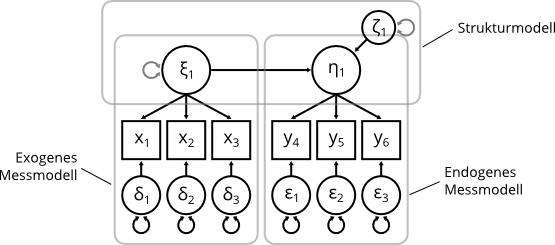
\includegraphics{images/sem.png}
  \caption{Strukturgleichungsmodell mit LISREL-Notation dargestellt. Messmodelle beschreiben einen Faktor und die zugehörigen Indikatoren, Strukturmodelle beschreiben die Zusammenhänge zwischen den Faktoren.}
  \label{img:sem}
\end{figure}

\paragraph*{Annahmen}

Die Annahmen des \emph{Messmodells} sind:

\begin{compactitem}
\item $\mathbb{E} [\boldsymbol\eta] = 0$, $\mathbb{E} [\boldsymbol\xi] = 0$
\item $\mathbb{E} [\boldsymbol\epsilon] = 0$, $\mathbb{E} [\boldsymbol\delta] = 0$
\item $\boldsymbol\epsilon$ unkorreliert mit $\boldsymbol\eta$, $\boldsymbol\xi$ und $\boldsymbol\delta$
\item $\boldsymbol\delta$ unkorreliert mit $\boldsymbol\eta$, $\boldsymbol\xi$ und $\boldsymbol\epsilon$
\end{compactitem}

Ebenso lauten die Annahmen des \emph{Strukturmodells}:

\begin{compactitem}
\item $\mathbb{E} [\boldsymbol\eta] = 0$, $\mathbb{E} [\boldsymbol\xi] = 0$, $\mathbb{E} [\boldsymbol\zeta] = 0$
\item $\boldsymbol\zeta$ unkorreliert mit $\boldsymbol\xi$
\item $\mathbf{I}-\mathbf{B}$ nicht singulär
\end{compactitem}

\paragraph*{Exogenes Messmodell}

In Matrixschreibweise wird das exogene Messmodell wie folgt beschrieben:

\begin{equation}
\mathbf{X} = \boldsymbol{\Lambda \, \xi} + \boldsymbol\delta
\end{equation}

Ausgeschrieben ergibt sich:

\begin{equation}
\begin{pmatrix}x_1\\ \vdots\\ x_n\end{pmatrix} = 
\begin{pmatrix}\lambda_{11} & \hdots & \lambda_{1k}\\ \vdots & \ddots & \vdots \\ \lambda_{n1} & \hdots & \lambda_{nk} \end{pmatrix}
\begin{pmatrix}\xi_1\\ \vdots\\ \xi_k\end{pmatrix} +
\begin{pmatrix}\delta_1\\ \vdots\\ \delta_n\end{pmatrix}
\end{equation}

Dabei ist $n$ die Anzahl der Indikatoren und $k$ die Anzahl der Faktoren. Sollen Einflüsse von bestimmten Indikatoren nur von bestimmten Faktoren berücksichtigt werden, so werden die entsprechenden Einträge Null gesetzt.

\subparagraph{Beispiel}

In diesem Fall liegen 4 Indikatoren und 2 exogene Faktoren vor. Jeweils nur 2 Indikatoren laden auf einen der exogenen Faktoren. D.h. $x_1 \wedge x_2 \to \xi_1$ mit $\delta_1$ und $\delta_2$, sowie $x_3 \wedge x_4 \to \xi_2$ mit $\delta_3$ und $\delta_4$. Das Modell wird wie folgt formuliert:

\begin{equation}
\begin{pmatrix}x_1\\ x_2\\ x_3\\ x_4\end{pmatrix} = 
\begin{pmatrix}\lambda_{11} & 0\\ \lambda_{21} & 0 \\ 0 & \lambda_{32}\\ 0 & \lambda_{42} \end{pmatrix}
\begin{pmatrix}\xi_1\\ \xi_2\end{pmatrix} +
\begin{pmatrix}\delta_1\\ \delta_2\\ \delta_3\\ \delta_4\end{pmatrix}
\end{equation}

\paragraph*{Endogenes Messmodell}

In Matrixschreibweise wird das endogene Messmodell wie folgt beschrieben:

\begin{equation}
\mathbf{Y} = \boldsymbol{\Lambda \, \eta} + \boldsymbol\epsilon
\end{equation}

Ausgeschrieben ergibt sich:

\begin{equation}
\begin{pmatrix}y_1\\ \vdots\\ y_n\end{pmatrix} = 
\begin{pmatrix}\lambda_{11} & \hdots & \lambda_{1k}\\ \vdots & \ddots & \vdots \\ \lambda_{n1} & \hdots & \lambda_{nk} \end{pmatrix}
\begin{pmatrix}\eta_1\\ \vdots\\ \eta_k\end{pmatrix} +
\begin{pmatrix}\epsilon_1\\ \vdots\\ \epsilon_n\end{pmatrix}
\end{equation}

\paragraph*{Strukturmodell}

Das Strukturmodell beschreibt die Zusammenhänge der Faktoren. Für den Spezialfall, dass ausschließlich der Zusammenhang zwischen exogenen Faktoren und endogene Faktor angegeben werden soll, wobei ein Faktor nicht als exogener und endogener Faktor gleichzeitig auftritt, lautet das Modell in Matrixschreibweise:

\begin{equation}
\boldsymbol\eta = \boldsymbol{\Gamma \xi} + \boldsymbol\zeta
\end{equation}

Ausgeschrieben ergibt sich:

\begin{equation}
\begin{pmatrix}\eta_1\\ \vdots\\ \eta_n\end{pmatrix} = 
\begin{pmatrix}\gamma_{11} & \hdots & \gamma_{1k}\\ \vdots & \ddots & \vdots \\ \gamma_{n1} & \hdots & \gamma_{nk} \end{pmatrix}
\begin{pmatrix}\xi_1\\ \vdots\\ \xi_k\end{pmatrix} +
\begin{pmatrix}\zeta_1\\ \vdots\\ \zeta_n\end{pmatrix}
\end{equation}

Dabei ist $n$ die Anzahl der endogenen Faktoren und $k$ die Anzahl der exogenen Faktoren.

Wenn endogene Variablen $\eta$ wieder auf endogene Variablen wirken (also eine Variable endogene und exogene Variable gleichzeitig ist), dann wird $\eta$ wieder auf der rechten Seite der Gleichung eingebracht und wir können das allgemeine Strukturmodell formulieren:

\begin{equation}
\label{eq:structmodel}
\boldsymbol\eta = \boldsymbol{\Gamma \xi} + \boldsymbol{B \eta} + \boldsymbol\zeta
\end{equation}

Ausgeschrieben ergibt sich:

\begin{equation}
\begin{pmatrix}\eta_1\\ \vdots\\ \eta_n\end{pmatrix} = 
\begin{pmatrix}\gamma_{11} & \hdots & \gamma_{1k}\\ \vdots & \ddots & \vdots \\ \gamma_{n1} & \hdots & \gamma_{nk} \end{pmatrix}
\begin{pmatrix}\xi_1\\ \vdots\\ \xi_k\end{pmatrix} +
\begin{pmatrix}\beta_{11} & \hdots & \beta_{1k}\\ \vdots & \ddots & \vdots \\ \beta_{n1} & \hdots & \beta_{nk} \end{pmatrix}
\begin{pmatrix}\eta_1\\ \vdots\\ \eta_h\end{pmatrix} +
\begin{pmatrix}\zeta_1\\ \vdots\\ \zeta_n\end{pmatrix}
\end{equation}

Dabei ist $n$ die Anzahl der endogenen Faktoren, die am Ende betrachtet werden, $k$ die Anzahl der exogenen Faktoren und $h$ die Anzahl der endogenen Faktoren, die wieder als exogene Faktoren wirken.

\subparagraph{Beispiele: Spezialfall}

Beispiel mit zwei exogenen Faktoren $\xi$ auf einen endogenen Faktor $\eta$ (d.h. $\xi_1 \wedge \xi_2 \to \eta$), wobei die $\xi$ die Indikatoren $x$ besitzen:

\begin{equation}
\eta = \begin{pmatrix}\gamma_1 & \gamma_2\end{pmatrix} \begin{pmatrix}\xi_1\\ \xi_2\end{pmatrix} + \zeta
\end{equation}

Beispiel mit zwei exogenen Faktoren $\xi$ und zwei endogenen Faktoren $\eta$, wobei $\xi_1 \to \eta_1$ und $\xi_2 \to \eta_2$:

\begin{equation}
\begin{pmatrix}\eta_1\\ \eta_2\end{pmatrix} =
\begin{pmatrix}\gamma_{11} & 0\\ 0 & \gamma_{22}\end{pmatrix}
\begin{pmatrix}\xi_1\\ \xi_2\end{pmatrix} +
\begin{pmatrix}\zeta_1\\ \zeta_2\end{pmatrix}
\end{equation}

\subparagraph{Beispiel: Allgemeiner Fall}

Als Beispiel sollen wieder zwei exogene $\xi$ und zwei endogene $\eta$ betrachtet werden. Dabei soll zusätzlich zu den Zusammenhängen $\xi_1 \to \eta_1$ und $\xi_2 \to \eta_2$ (wie im vorigen Beispiel) auch der Zusammenhang zwischen zwei endogenen Faktoren $\eta_1 \to \eta_2$ gelten.

\begin{equation}
\begin{pmatrix}\eta_1\\ \eta_2\end{pmatrix} =
\begin{pmatrix}\gamma_{11} & 0\\ 0 & \gamma_{22}\end{pmatrix}
\begin{pmatrix}\xi_1\\ \xi_2\end{pmatrix} +
\begin{pmatrix}0 & 0\\ \beta_{21} & 0\end{pmatrix}
\begin{pmatrix}\eta_1\\ \eta_2\end{pmatrix} +
\begin{pmatrix}\zeta_1\\ \zeta_2\end{pmatrix}
\end{equation}

\subsubsection{Modellimplizierte Kovarianzmatrix}

\paragraph*{Allgemeine Kovarianzen}

Zusammenhänge zwischen den Variablen können in einer Kovarianzmatrix beschrieben werden.

Im \emph{Messmodell} werden zusammenhänge zwischen den Fehlertermen betrachtet. Die Kovarianzmatrixen sind:

\begin{compactitem}
\item $\boldsymbol\Theta_{\boldsymbol\delta} = \mathbb{E} \left[ \boldsymbol{\delta\delta}^T \right]$
\item $\boldsymbol\Theta_{\boldsymbol\epsilon} = \mathbb{E} \left[ \boldsymbol{\epsilon\epsilon}^T \right]$
\end{compactitem}

Für unkorrelierte Fehler gilt:

\begin{equation}
\boldsymbol\Theta_{\boldsymbol\delta} =
\begin{pmatrix}
\sigma^2_{\delta_1} & 0 & 0\\
0 & \ddots & 0\\
0 & 0 & \sigma^2_{\delta_n}
\end{pmatrix}
\quad,\qquad
\boldsymbol\Theta_{\boldsymbol\epsilon} =
\begin{pmatrix}
\sigma^2_{\epsilon_1} & 0 & 0\\
0 & \ddots & 0\\
0 & 0 & \sigma^2_{\epsilon_n}
\end{pmatrix}
\end{equation}

Im \emph{Strukturmodell} werden folgende Kovarianzmatrizen betrachtet:

\begin{compactitem}
\item $\boldsymbol\Phi = \mathbb{E} \left[ \boldsymbol{\xi\xi}^T \right]$
\item $\boldsymbol\Psi = \mathbb{E} \left[ \boldsymbol{\zeta\zeta}^T \right]$
\end{compactitem}

\subparagraph{Beispiel: Exogene Faktoren}

Werden z.B. zwei exogene Faktoren $\xi_1$ und $\xi_2$ betrachtet, so ergibt sich die Kovarianzmatrix wie folgt:

\begin{equation}
\boldsymbol\Phi =
\begin{pmatrix}
Var(\xi_1) & Cov(\xi_1,\xi_2)\\
Cov(\xi_2,\xi_1) & Var(\xi_2)
\end{pmatrix} =
\begin{pmatrix}
\phi_{11} & \phi_{12}\\
\phi_{21} & \phi_{22}
\end{pmatrix}
\end{equation}

Wobei $\phi_{12}$ = $\phi_{21}$, d.h. eine Kovarianzmatrix ist symmetrisch, da die einzelnen Kovarianzen der Zufallsvariablen symmetrisch sind, d.h. $Cov(X,Y) = Cov(Y,X)$.

\subparagraph{Beispiel: Endogene Faktoren}

Analog zu den exogenen Faktoren, ergibt sich die Kovarianzmatrix für zwei endogene Faktoren $\zeta_1$ und $\zeta_2$ wie folgt:

\begin{equation}
\boldsymbol\Psi =
\begin{pmatrix}
Var(\zeta_1) & Cov(\zeta_1,\zeta_2)\\
Cov(\zeta_2,\zeta_1) & Var(\zeta_2)
\end{pmatrix} =
\begin{pmatrix}
\psi_{11} & \psi_{12}\\
\psi_{21} & \psi_{22}
\end{pmatrix}
\end{equation}

Auch hier gilt Symmetrie und somit $\psi_{12}$ = $\psi_{21}$.

\paragraph*{Modellimplizierte Kovarianzmatrix}

In der Einführung des aktuellen Abschnitts wurde bereits deutlich, dass es das Ziel ist die Abweichung zwischen der \textbf{modellimplizierten Kovarianzmatrix} $\boldsymbol{\Sigma(\theta)}$ und der \emph{empirischen Kovarianzmatrix} $\boldsymbol\Sigma$ zu minimiert. Zur Formulierung der modellimplizierten Kovarianzmatrix beginnen wir mit vier Komponenten der Matrix:

\begin{equation}
\boldsymbol{\Sigma(\theta)} = \boldsymbol\Sigma
\begin{pmatrix}
\boldsymbol\Sigma_{\mathbf{YY}}(\boldsymbol\theta) & \boldsymbol\Sigma_{\mathbf{YX}}(\boldsymbol\theta)\\
\boldsymbol\Sigma_{\mathbf{XY}}(\boldsymbol\theta) & \boldsymbol\Sigma_{\mathbf{XX}}(\boldsymbol\theta)
\end{pmatrix}
\end{equation}

\subparagraph*{1. Exogener Teil}

\begin{equation}
\label{eq:kovar-xx}
\begin{split}
\boldsymbol\Sigma_{\mathbf{XX}}(\boldsymbol\theta) &= \mathbb{E} \left[ \mathbf{XX}^T \right] = \mathbb{E} \left[ (\boldsymbol\Lambda_{\mathbf{X}} \boldsymbol\xi + \boldsymbol\delta) (\boldsymbol\Lambda_{\mathbf{X}} \boldsymbol\xi + \boldsymbol\delta)^T \right]\\
&= \mathbb{E} \left[ \boldsymbol\Lambda_{\mathbf{X}} \boldsymbol\xi (\boldsymbol\Lambda_{\mathbf{X}} \boldsymbol\xi)^T + \boldsymbol\Lambda_{\mathbf{X}} \boldsymbol\xi \boldsymbol\delta^T + \boldsymbol\delta (\boldsymbol\Lambda_{\mathbf{X}} \boldsymbol\xi)^T +\boldsymbol{\delta\delta}^T \right]\\
&= \mathbb{E} \left[ \boldsymbol\Lambda_{\mathbf{X}} \boldsymbol\xi \boldsymbol\xi^T \boldsymbol\Lambda_{\mathbf{X}}^T + \boldsymbol\Lambda_{\mathbf{X}} \boldsymbol\xi \boldsymbol\delta^T + \boldsymbol\delta \boldsymbol\xi^T \boldsymbol\Lambda_{\mathbf{X}}^T +\boldsymbol{\delta\delta}^T \right]\\
&= \boldsymbol\Lambda_{\mathbf{X}} \mathbb{E} \left[ \boldsymbol{\xi\xi}^T \right] \boldsymbol\Lambda_{\mathbf{X}}^T + 0 + 0 + \mathbb{E} \left[ \boldsymbol{\delta\delta}^T \right]\\
&= \boldsymbol\Lambda_{\mathbf{X}} \boldsymbol\Phi \boldsymbol\Lambda_{\mathbf{X}}^T + \boldsymbol\Theta_{\boldsymbol\delta}
\end{split}
\end{equation}

Die letzten Schritte folgen aus der Annahme $\mathbb{E}[\boldsymbol\xi] = 0$ und den Kovarianzmatrizen für die Fehler.

\subparagraph*{2. Endogener Teil}

\begin{equation}
\label{eq:endo-1}
\begin{split}
\boldsymbol\Sigma_{\mathbf{YY}}(\boldsymbol\theta) &= \mathbb{E} \left[ \mathbf{YY}^T \right] =  \mathbb{E} \left[ (\boldsymbol\Lambda_{\mathbf{Y}} \boldsymbol\eta + \boldsymbol\epsilon) (\boldsymbol\Lambda_{\mathbf{Y}} \boldsymbol\eta + \boldsymbol\epsilon)^T \right]\\
&= \dots = \boldsymbol\Lambda_{\mathbf{Y}} \mathbb{E} \left[ \boldsymbol{\eta\eta}^T \right] \boldsymbol\Lambda_{\mathbf{Y}}^T + \boldsymbol\Theta_{\boldsymbol\epsilon}
\end{split}
\end{equation}

Der Erwartungswert $\mathbb{E} \left[ \boldsymbol{\eta\eta}^T \right]$ kann nicht zusammengefasst werden, da $\boldsymbol\eta$ auch als Funktion der exogenen Faktoren ausgedrückt werden kann. $\boldsymbol\eta$ muss zunächst mit Hilfe der Strukturmodell-Gleichung~\ref{eq:structmodel} umgeformt werden. Wir beginnen mit:

\begin{subequations}
\begin{equation}
\boldsymbol\eta - \boldsymbol{B \eta} = \boldsymbol{\Gamma \xi} + \boldsymbol\zeta
\end{equation}
\begin{equation}
(\mathbf{I} - \mathbf{B}) \boldsymbol\eta = \boldsymbol{\Gamma \xi} + \boldsymbol\zeta
\end{equation}
\begin{equation}
\label{eq:eta}
\boldsymbol\eta = (\mathbf{I} - \mathbf{B})^{-1} \boldsymbol{\Gamma \xi} + \boldsymbol\zeta
\end{equation}
\end{subequations}

Nun kann der Erwartungswert $\mathbb{E} \left[ \boldsymbol{\eta\eta}^T \right]$ mit Gleichung~\ref{eq:eta} bestimmt werden mit:

\begin{equation}
\begin{split}
\mathbb{E} \left[ \boldsymbol{\eta\eta}^T \right] &= \mathbb{E} \left[ \left( (\mathbf{I} - \mathbf{B})^{-1} (\boldsymbol{\Gamma \xi} + \boldsymbol\zeta) \right) \left( (\mathbf{I} - \mathbf{B})^{-1} (\boldsymbol{\Gamma \xi} + \boldsymbol\zeta) \right)^T \right]\\
&= \mathbb{E} \left[ \left( (\mathbf{I} - \mathbf{B})^{-1} (\boldsymbol{\Gamma \xi} + \boldsymbol\zeta) \right) \left( ((\boldsymbol{\Gamma \xi})^T + \boldsymbol\zeta^T) (\mathbf{I} - \mathbf{B})^{{-1}^T} \right) \right]\\
&= \mathbb{E} \left[ (\mathbf{I} - \mathbf{B})^{-1} (\boldsymbol{\Gamma \xi} + \boldsymbol\zeta) ( \boldsymbol\xi^T \boldsymbol\Gamma^T + \boldsymbol\zeta^T) (\mathbf{I} - \mathbf{B})^{{-1}^T} \right]\\
&= (\mathbf{I} - \mathbf{B})^{-1} (\boldsymbol\Gamma \mathbb{E} \left[ \boldsymbol\xi \boldsymbol\xi^T \right] \boldsymbol\Gamma^T + \mathbb{E} \left[ \boldsymbol\zeta \boldsymbol\zeta^T \right]) (\mathbf{I} - \mathbf{B})^{{-1}^T}\\
&= (\mathbf{I} - \mathbf{B})^{-1} (\boldsymbol\Gamma \boldsymbol\Phi \boldsymbol\Gamma^T + \boldsymbol\Psi) (\mathbf{I} - \mathbf{B})^{{-1}^T}\\
\end{split}
\end{equation}

Einsetzen in Gleichung~\ref{eq:endo-1} liefert:

\begin{equation}
\label{eq:kovar-yy}
\boldsymbol\Sigma_{\mathbf{YY}}(\boldsymbol\theta) = \boldsymbol\Lambda_{\mathbf{Y}} (\mathbf{I} - \mathbf{B})^{-1} (\boldsymbol\Gamma \boldsymbol\Phi \boldsymbol\Gamma^T + \boldsymbol\Psi) (\mathbf{I} - \mathbf{B})^{{-1}^T} \boldsymbol\Lambda_{\mathbf{Y}}^T + \boldsymbol\Theta_{\boldsymbol\epsilon}
\end{equation}

\subparagraph*{3. Kovarianzen zwischen endogenem und exogenem Anteil}

Die Kovarianzen können mit Hilfe analoger Berechnung erhalten werden. Für $\boldsymbol\Sigma_{\mathbf{YX}}(\boldsymbol\theta)$ gilt:

\begin{equation}
\label{eq:kovar-yx}
\boldsymbol\Sigma_{\mathbf{YX}}(\boldsymbol\theta) = \boldsymbol\Lambda_{\mathbf{Y}} (\mathbf{I} - \mathbf{B})^{-1} \boldsymbol\Gamma \boldsymbol\Phi \boldsymbol\Lambda_{\mathbf{X}}^T
\end{equation}

Der letzte Anteil ergibt sich durch transponieren $\boldsymbol\Sigma_{\mathbf{XY}}(\boldsymbol\theta) = \boldsymbol\Sigma_{\mathbf{YX}}(\boldsymbol\theta)^T$, damit folgt:

\begin{equation}
\label{eq:kovar-xy}
\boldsymbol\Sigma_{\mathbf{XY}}(\boldsymbol\theta) = \boldsymbol\Lambda_{\mathbf{X}} \boldsymbol\Phi \boldsymbol\Gamma^T (\mathbf{I} - \mathbf{B})^{{-1}^T} \boldsymbol\Lambda_{\mathbf{Y}}^T
\end{equation}

\subparagraph*{Resultat}

Die modellimplizierten Kovarianzmatrix berechnet sich abschließend mit Gleichungen~\ref{eq:kovar-xx}, \ref{eq:kovar-yy}, \ref{eq:kovar-yx} und \ref{eq:kovar-xy} wie folgt:

\begin{equation}
\boldsymbol{\Sigma(\theta)} = \boldsymbol\Sigma
\begin{pmatrix}
\boldsymbol\Lambda_{\mathbf{Y}} (\mathbf{I} - \mathbf{B})^{-1} (\boldsymbol\Gamma \boldsymbol\Phi \boldsymbol\Gamma^T + \boldsymbol\Psi) (\mathbf{I} - \mathbf{B})^{{-1}^T} \boldsymbol\Lambda_{\mathbf{Y}}^T + \boldsymbol\Theta_{\boldsymbol\epsilon}
&
\boldsymbol\Lambda_{\mathbf{Y}} (\mathbf{I} - \mathbf{B})^{-1} \boldsymbol\Gamma \boldsymbol\Phi \boldsymbol\Lambda_{\mathbf{X}}^T
\\
\boldsymbol\Lambda_{\mathbf{X}} \boldsymbol\Phi \boldsymbol\Gamma^T (\mathbf{I} - \mathbf{B})^{{-1}^T} \boldsymbol\Lambda_{\mathbf{Y}}^T
&
\boldsymbol\Lambda_{\mathbf{X}} \boldsymbol\Phi \boldsymbol\Lambda_{\mathbf{X}}^T + \boldsymbol\Theta_{\boldsymbol\delta}
\end{pmatrix}
\end{equation}

\subsubsection{Exkurs: RAM-Notation}

Neben der \emph{LISREL}-Notation gibt es weitere Methoden zur Beschreibung von Strukturgleichungsmodellen. Ähnlich wie bei LISREL sind diese häufig an Software gebunden. Übliche Notationen sind (in Klammern die zugehörige Software):

\begin{compactitem}
\item LISREL (LISREL)
\item Bentler-Weeks (EQS)
\item RAM (RAMONA)
\end{compactitem}

Im Folgenden wird eine Alternative zur LISREL-Notation, die \textbf{RAM-Notation} betrachtet. Unterschieden wird dort nur zwischen drei Matrizen $\mathbf{S}$, $\mathbf{A}$ und $\mathbf{F}$ und einem Vektor $\mathbf{m}$. Die Matrizen und der transponierte Vektor enthalten in den ersten Spalten die latenten Variablen, die letzten Spalten enthalten die beobachteten Variablen. Das Beispiel aus Abbildung~\ref{img:sem} würde in RAM-Notation wie folgt definiert werden:

\begin{equation}
\mathbf{S} = \begin{bmatrix}
\phi & 0 & 0 & 0 & 0 & 0 & 0 & 0\\
0 & \psi & 0 & 0 & 0 & 0 & 0 & 0\\
0 & 0 & \sigma^2_{\delta_1} & 0 & 0 & 0 & 0 & 0\\
0 & 0 & 0 & \sigma^2_{\delta_2} & 0 & 0 & 0 & 0\\
0 & 0 & 0 & 0 & \sigma^2_{\delta_3} & 0 & 0 & 0\\
0 & 0 & 0 & 0 & 0 & \sigma^2_{\epsilon_1} & 0 & 0\\
0 & 0 & 0 & 0 & 0 & 0 & \sigma^2_{\epsilon_2} & 0\\
0 & 0 & 0 & 0 & 0 & 0 & 0 & \sigma^2_{\epsilon_3}
\end{bmatrix}\;,\qquad
\mathbf{A} = \begin{bmatrix}
0 & 0 & 0 & 0 & 0 & 0 & 0 & 0\\
\gamma & 0 & 0 & 0 & 0 & 0 & 0 & 0\\
\lambda_1 & 0 & 0 & 0 & 0 & 0 & 0 & 0\\
\lambda_2 & 0 & 0 & 0 & 0 & 0 & 0 & 0\\
\lambda_3 & 0 & 0 & 0 & 0 & 0 & 0 & 0\\
0 & \lambda_4 & 0 & 0 & 0 & 0 & 0 & 0\\
0 & \lambda_5 & 0 & 0 & 0 & 0 & 0 & 0\\
0 & \lambda_6 & 0 & 0 & 0 & 0 & 0 & 0
\end{bmatrix}
\end{equation}

Dabei bezeichnen $\phi$ und $\psi$ die (Ko-)Varianzen der latenten Variablen und $\sigma^2$ die der beobachteten (manifesten) Variablen. Diese Kovarianzmatrix $\mathbf{S}$ ist \emph{symmetrisch}.

Die $\lambda$ entstammen der Faktorladungsmatrix $\boldsymbol\Lambda$. $\gamma$ ist der Zusammenhang zwischen den Faktoren $\xi$ und $\eta$. Diese Zusammehangsmatrix $\mathbf{A}$ ist \emph{asymmetrisch}.

Die Matrizen $\mathbf{F}$ bezeichnet eine Filter-Matrix, der Vektor $\mathbf{m}$ gibt die Mittelwerte an. Beide werden hier nicht weiter betrachtet.

\subsubsection{Software}

\begin{compactitem}
\item $\boldsymbol\Omega$\textbf{nyx}: Sehr benutzerfreundlich für einfache Modelle
\item \textbf{OpenMX}: Sehr komplex, Programmierkenntnisse nötig
\item \textbf{MPlus}: Wenige Befehle reichen aus um komplexe Modelle zu berechnen, trifft viele Default-Entscheidungen
\item \textbf{LISREL}: Klassiker, von dem auch die Notation abgelietet ist
\item Weitere: \textbf{R}, \textbf{AMOS}, \textbf{SAS}, \textbf{Mx}, \textbf{sem()}, \textbf{EQS}, \textbf{lavaan}
\end{compactitem}

\subparagraph{Beispiele: Onyx}

\begin{figure}
  \centering
  \captionsetup{justification=centering}
  \begin{subfigure}[b]{0.48\textwidth}
    \centering
    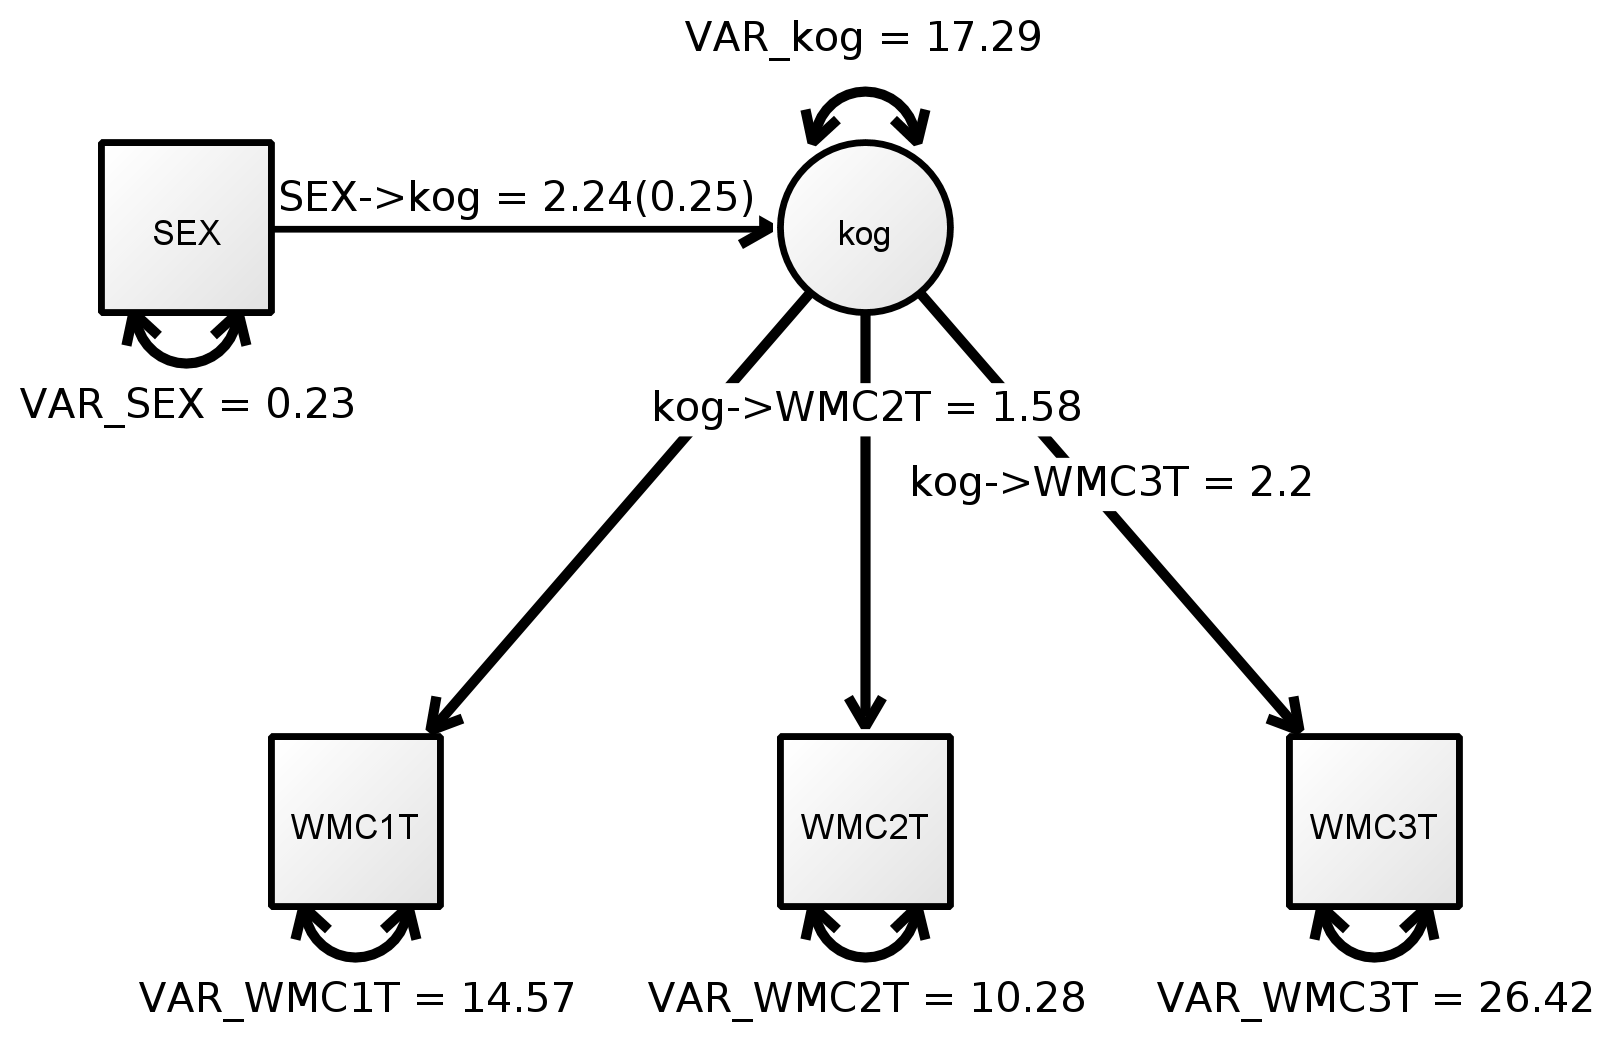
\includegraphics[width=0.85\textwidth]{images/onyx/onyx_kog.png}
    \caption{Effekt von Geschlecht auf kognitive Leistungsfähigkeit}
    \label{img:onyx-kog}
  \end{subfigure}
  \begin{subfigure}[b]{0.48\textwidth}
    \centering
    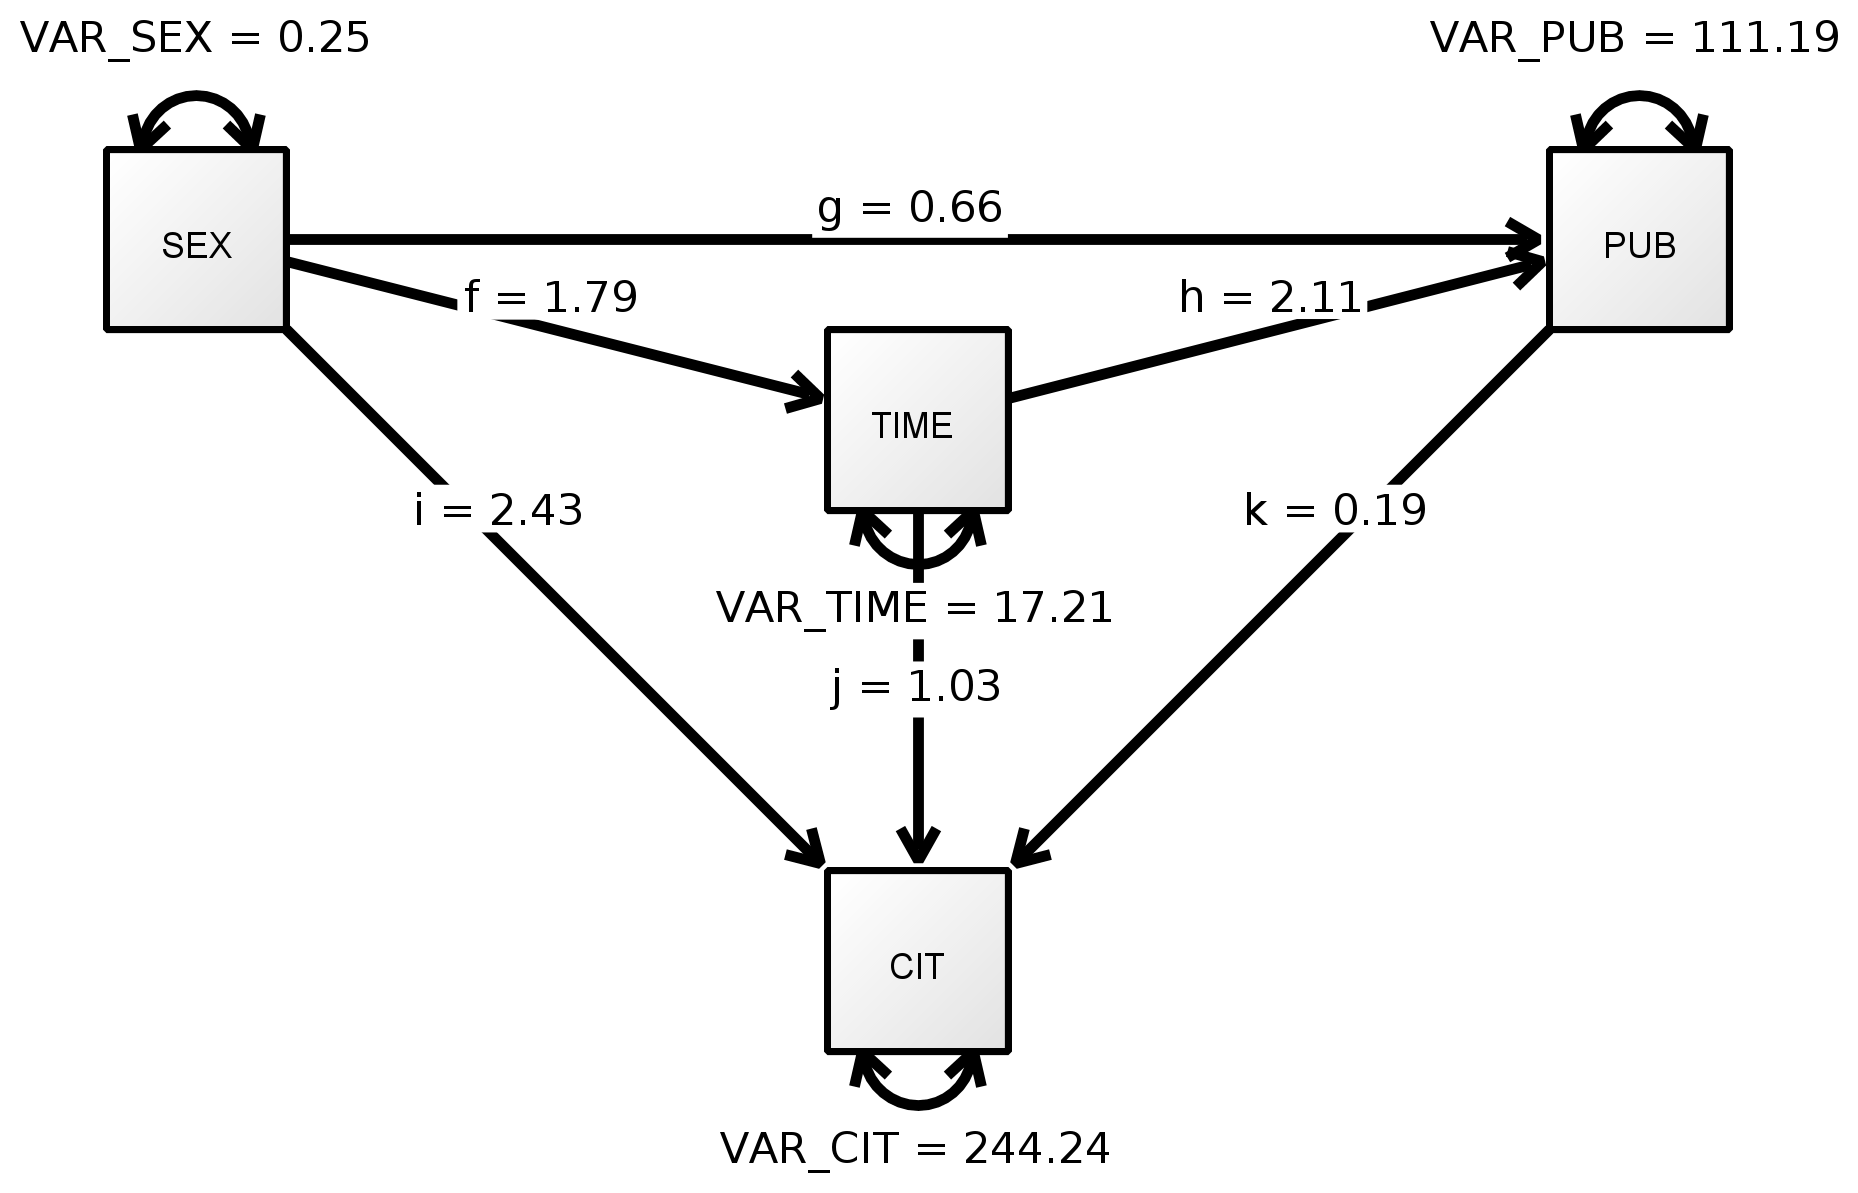
\includegraphics[width=0.85\textwidth]{images/onyx/onyx_cit.png}
    \caption{Effekte auf Anzahl der Zitationen von Professoren}
    \label{img:onyx-cit}
  \end{subfigure}
  \caption{Strukturgleichungsmodelle mit Onyx}
\end{figure}

Beispiel 1: Einfluss des Geschlechts auf kognitive Leistungsfähigkeit. Dabei ist die kognitive Leistungsfähigkeit ein Faktor bzw. eine latente Variable, welcher durch drei beobachtete Variablen beschrieben wird. Es wird ein \emph{Messmodell} (Faktor) und ein \emph{Strukturodell} verwendet (Einfluss Geschlecht auf kognitive Leistung). Das Beispiel ist in Abbildung~\ref{img:onyx-kog} dargestellt. Eine Erhöhung im Geschlecht um $1$, führt zu einer erhöhten Leistung um $2,24$ (bzw. standardisiert $0,25$).

Beispiel 2: Auch das \emph{Pfadmodell} mit den Professorengehältern lässt sich mit Onyx modellieren. Das Beispiel ist in Abbildung~\ref{img:onyx-cit} dargestellt. Eine Erhöhung um $1$ des Geschlechts erhöht bspw. die Anzahl der Zitationen um $2,43$ und die Anzahl der Publikationen um $0,66$.

\subsubsection*{Begriffe}

\fbox{\begin{minipage}{\textwidth}
Multiple vs. Multivariate Modelle, Modellimplizierte Kovarianzmatrix, Empirische Kovarianzmatrix, LISREL, Messmodell, Strukturmodell, Notation, Variablen der SEM, Annahmen, Exogenes/Endogenes Messmodell, Alternative Notationen, RAM, Software, Interpretation
\end{minipage}}

\subsection{Angewandte Strukturgleichungsmodelle}

\subsubsection{Modellspezifikation}

Wir spezifizieren Strukuturgleichungsmodelle mit der eingeführten LISREL-Notation. Die Notationsregel ist analog zu Pfaddiagrammen.

\subsubsection{Modellidentifikation}

Für ein spezifiziertes Modell kann die \emph{empirische Kovarianzmatrix} $\boldsymbol\Sigma$ angegeben werden, der Parameter $\boldsymbol\theta$ kann anschließend durch Minimierung bzgl. der \emph{modellimplizierte Kovarianzmatrix} $\boldsymbol\Sigma(\boldsymbol\theta)$ gewonnen werden.

\begin{equation}
\hat{\boldsymbol\theta} = \underset{\boldsymbol\theta}{arg\,min} \left[ \boldsymbol\Sigma,\,\boldsymbol\Sigma(\boldsymbol\theta) \right]
\end{equation}

Die \emph{Anzahl der unbekannten Parameter} $\boldsymbol\theta$ in der \emph{modellimplizierten Kovarianzmatrix} $\boldsymbol\Sigma(\boldsymbol\theta)$ und die \emph{Anzahl der bekannten Varianzen und Kovarianzen} in der \emph{empirische Kovarianzmatrix} $\boldsymbol\Sigma$ können sich unterscheiden. Dies führt bei der Minimierung zu Resultaten, die wie folgt unterschieden werden können:

\begin{tabular}{llp{11cm}}
\textbf{Typ} & \textbf{Freiheitsg.} & \textbf{Beschreibung}\\
\hline
\textbf{just identified} & $df = 0$ & Es gibt genau eine Möglichkeit alle Parameter $\boldsymbol\theta$ als eineindeutige Funktion von $\boldsymbol\Sigma$ zu beschreiben.\\
\textbf{over identified} & $df > 0$ & Es gibt mehrere Möglichkeiten alle Parameter $\boldsymbol\theta$ als eineindeutige Funktion von $\boldsymbol\Sigma$ zu beschreiben.\\
\textbf{under identified} & $df < 0$ & Es gibt keine Möglichkeiten alle Parameter $\boldsymbol\theta$ als eineindeutige Funktion von $\boldsymbol\Sigma$ zu beschreiben (in diesem Fall existiert keine Lösung).
\end{tabular}

Bestimmte Annahmen bzw. Beschränkungen (\textbf{constraints}) sind nötig, um eine Berechnung der Modelle zu gewährleisten. Zwei wichtige Constraints sind:

\begin{compactenum}
\item Die Diagonale von $\mathbf{B}$ muss Null sein. Variablen dürfen keine Effekte auf sich selbst haben.
\item Das Regressionsgewicht der latenten Variablen $\boldsymbol\xi$, $\boldsymbol\eta$, $\boldsymbol\zeta$, $\boldsymbol\delta$ und $\boldsymbol\epsilon$ wird auf $1$ fixiert. Latente Variablen können nicht direkt beobachtet werden, ihnen muss eine Skala zugewiesen werden.
\end{compactenum}

\paragraph*{Skalierung}

Aus der zweiten Annahme folgt eine notwendige Skalierung. Bisher wurde die Skala einer anderen Variablen übernommen, indem der Effekt auf $1$ fixiert wurde (siehe Abbildung~\ref{img:skala-x}). Es gilt:

\begin{equation}
\begin{pmatrix}
x_1\\ x_2\\ x_3
\end{pmatrix} = 
\begin{pmatrix}
1 & 0 & 0\\
0 & 1 & 0\\
0 & 0 & 1
\end{pmatrix}
\begin{pmatrix}
\delta_1\\ \delta_2\\ \delta_3
\end{pmatrix}
\end{equation}

Dabei wird die mittlere Matrix (Einheitsmatrix) als \textbf{Skalierungsmatrix} bezeichnet.

Um auch die \emph{latenten Variablen} zu skalieren, gibt es zwei Möglichkeiten

\begin{compactitem}
\item Fixierung des Effekts der ersten manifesten Variable auf $1$ (prinzipiell kann jede Variable gewählt werden), siehe Abbildung~\ref{img:skala-latent}
\item Fixierug der Varianz einer latenten Variablen $\phi$, siehe Abbildung~\ref{img:skala-varianz}
\end{compactitem}

\begin{figure}
  \centering
  \captionsetup{justification=centering}
  \begin{subfigure}[b]{0.32\textwidth}
    \centering
    
\includegraphics[width=0.6\textwidth]{images/sem/skala-x.png}
    \caption{Skalierung der manifesten Variablen durch Fixierung der Effekt auf $x$ auf $1$.}
    \label{img:skala-x}
  \end{subfigure}
  \begin{subfigure}[b]{0.32\textwidth}
    \centering
    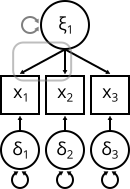
\includegraphics[width=0.6\textwidth]{images/sem/skala-latent.png}
    \caption{Skalierung der latenten Variablen durch Fixierung des Effektes einer manifesten Variablen auf $1$.}
    \label{img:skala-latent}
  \end{subfigure}
  \begin{subfigure}[b]{0.32\textwidth}
    \centering
    
\includegraphics[width=0.6\textwidth]{images/sem/skala-varianz.png}
    \caption{Skalierung der latenten Variablen durch Fixierung der Varianz $\phi$. Alternative für~\ref{img:skala-latent}.}
    \label{img:skala-varianz}
  \end{subfigure}
  \caption{Skalierung von Variablen}
  \label{img:skala}
\end{figure}

\paragraph*{Identifikationsregeln}

Das in Abbildung~\ref{img:skala} beschriebene Modell ist \emph{just identified}. Die Identifikation eines Modells wird gezeigt, indem \emph{algebraisch} nachgewiesen wird, dass es genau eine Möglichkeit gibt alle Parameter $\boldsymbol\theta$ als eineindeutige Funktion von von $\boldsymbol\Sigma$ zu beschreiben (vgl. Lösungstyp \emph{just identified}). Dieser Beweis ist bei größeren Modell jedoch sehr aufwändig.

Um einen Beweis umgehen zu können, können Identifikationsregeln formuliert werden.

\begin{tabular}{lllcc}
\textbf{Regel} & \textbf{Anwendung} & \textbf{Bedingung} & \textbf{Notw.} & \textbf{Hinr.}\\
\hline
t-Rule & Alle & $t \le \frac{1}{2}(p+q)(p+q+1)$ & ja & nein\\
Null $\mathbf{B}$ rule & Beob. Var. & $\mathbf{B} = 0$ & nein & ja\\
Recursive Rule & Beob. Var. & $\mathbf{B}$ Dreiecksmatrix, $\boldsymbol \Psi$ Diagonalmatrix \vspace*{0.3cm} & nein & ja\\
Three-Indicator-Rule & Messmodelle & \pbox{7.5cm}{$n \ge 1$, $\boldsymbol \Theta$ Diagonalmatrix\\ Mind. ein Elem. pro Zeile von $\boldsymbol \Lambda$ ist nicht Null\\ Drei oder mehr Indikatoren pro Faktor}\vspace*{0.3cm} & nein & ja\\
\pbox{4cm}{Two-Indicator-Rule\\ Regel 1} & Messmodelle & \pbox{7.5cm}{$n > 1$, $\boldsymbol \Theta$ Diagonalmatrix\\ $\phi_{ij} \neq 0 \;\forall\; i,j$\\ Mind. ein Elem. pro Zeile von $\boldsymbol \Lambda$ ist nicht Null\\ Zwei oder mehr Indikatoren pro Faktor}\vspace*{0.3cm} & nein & ja\\
\pbox{4cm}{Two-Indicator-Rule\\ Regel 2} & Messmodelle & \pbox{7.5cm}{$n > 1$, $\boldsymbol \Theta$ Diagonalmatrix\\ $\phi_{ij} \neq 0$ für mind. ein Paar mit $i \neq j$\\ (In jeder Zeile von $\phi_{ij}$ mind. ein Elem. nicht Null)\\ Mind. ein Elem. pro Zeile von $\boldsymbol \Lambda$ ist nicht Null\\ Zwei oder mehr Indikatoren pro Faktor}\vspace*{0.3cm} & nein & ja\\
Two-Step-Rule & Allg. SEM & \pbox{7.5cm}{1. Ursprüngliches Modell in Messmodell umformulieren, eliminiere $\mathbf{B}$, $\boldsymbol \Lambda$ und $\boldsymbol \Psi$, Identifiziere Messmodell\\ 2. Identifiziere Strukturmodell (Annahme: Keine Messfehler der zu Grunde liegenden Beobachtungen)} & nein & ja
\end{tabular}

Bei der t-Rule entspricht $q$ der Anzahl der Indikatoren exogener latenter Variablen und $p$ der Anzahl der Indikatoren endogener latenter Variablen. $t$ ist die Anzahl der zu schätzenden Parameter.

Notwendige Bedingung bedeutet dabei: Tritt die Bedingung ein, so ist das Modell auf jeden Fall identifiziert. Aus einem identifizierten Modell folgt aber nicht, dass die Bedingung erfüllt ist.\\
Eine hinreichende Bedingung bedeutet: Ist das Modell identifiziert, so ist die Bedingung auf jeden Fall erfüllt. Aus einer erfüllten Bedingung folgt aber noch nicht, dass das Modell identifiziert ist.

Da es keine Bedingung gibt, die notwendig und hinreichend gleichzeitig ist, kann eine eindeutige Aussage nicht immer getroffen werden. Vor allem dann, wenn keine der Bedingungen zutrifft, muss das Modell daher nicht abgelehnt werden, es könnte immer noch lösbar sein. Folgende Regeln können helfen:

\begin{compactitem}
\item Identifikationsregeln treffen zu: Modell ist identifiziert
\item Keine Identifikationsregel trifft zu: Algebraische Lösung versuchen
\item Identifikationsregeln gibt Warnung: Weitere Indizien prüfen (z.B. positiv definite Hesse-Matrix)
\item Testen unterschiedlicher Startwerte für die numerische Berechnung. Sind die Ergebnisse immer wieder ähnlich, dann ist das Modell wahrscheinlich identifiziert.
\item Reproduzierte Kovarianzmatrix speichern und als Input für neue Schätzung verwenden. Bei einem identifizierten Modell sind die Parameter identisch.
\end{compactitem}

\subsubsection{Modellschätzung}

Nach der Identifikation erfolgt die \textbf{Schätzung} des Modells. Dabei wird die Distanz zwischen den Matrizen $\boldsymbol \Sigma$ und $\boldsymbol \Sigma (\boldsymbol \theta)$ minimiert. Zunächst muss die \textbf{Distanz} dafür definiert werden. Es werden vier Schätzverfahren betrachtet:

\paragraph*{1. Unweighted Least Squares (ULS)}

Bei der Methode der \textbf{Unweighted Least Squares} werden kleinsten Quadrate ungwichtet gebildet, analog zur Methode der kleinsten Quadrate (ordinary least squares) bei der linearen Regression (vgl. Abschnitt~\ref{sec:grund-reg}). Er kann für normalverteilte Variablen verwendet werden.

\begin{equation}
F_{ULS} = \frac{1}{2}\, \text{tr} \left[ \left( \boldsymbol \Sigma - \boldsymbol \Sigma (\boldsymbol \theta) \right)^2 \right]
\end{equation}

Die Differenz der beiden Matrizen ergibt die Residualmatrix, welche minimiert wird. Wegen der Symmetrie der Matrix, erhalten die Kovarianzen (sie kommen immer doppelt in der Matrix vor) ein größeres Gewicht.

\subparagraph*{Vorteile}

\begin{compactitem}
\item Einfach zu berechnen
\item Algebraische Lösung leichter zu ermitteln
\item Konsistenter Schätzer von $\boldsymbol \theta$
\end{compactitem}

\subparagraph*{Nachteile}

\begin{compactitem}
\item Effizientere Schätzer sind möglich
\item Nicht skaleninvariant und nicht skalenfrei
\item Verteilungsannahmen nötig (für Standardfehler und $\chi^2$-Teststatistiken)
\end{compactitem}

\paragraph*{2. Maximum Likelihood (ML)}

Der häufigst verwendete Schätzer ist der \textbf{Maximum Likelihood Schätzer}. Dabei wird $\theta$ so gewählt, dass die Wahrscheinlichkeit für das Auftreten der empirischen Kovarianzmatrix $\boldsymbol \Sigma$ maximal wahrscheinlich ist.

\begin{equation}
F_{ML} = \ln |\boldsymbol \Sigma ( \boldsymbol \theta )| + \text{tr} ( \boldsymbol{\Sigma\Sigma} (\boldsymbol \theta)^{-1} ) - \ln | \boldsymbol \Sigma | - (p+q)
\end{equation}

Dabei geben $p$ und $q$ die Anzahl der manifesten Variablen an. Es gilt $F_{ML} \to 0$ je plausibler der Parameter die empirische Kovarianzmatrix erklären kann.

Die Maximum Likelihood Methode wird unter der \emph{Annahme} normalverteilter Zufallsvariablen angewendet.

\subparagraph*{Lösungen}

Die Parameter werden über Ableiten und Nullsetzen gewonnen (und durch Prüfung der hinreichenden Bedingung, d.h. zweite Ableitung ist positiv definit). Da nur für einfache Modelle analytischen Lösungen existieren, werden meist numerische Optimierungsverfahren eingesetzt. Dabei gilt:

\textbf{1. Startwerte}: Es müssen günstige Startwerte gewählt werden. Dies kann erfolgen durch:

\begin{compactitem}
\item A priori Wissen (Theorie)
\item A priori nicht-iterative Verfahren (ULS)
\item OLS Regression für jede einzelne Gleichung
\item Einfaches probieren mehrerer Werte (Versuch und Irrtum)
\item Daumenregeln und Empfehlungen
\end{compactitem}

\textbf{2. Optimierungsverfahren}: Es muss ein geeignetes Optimierungsverfahren gefunden werden. In einfachen Fällen liefert das Verfahren eine monotone Funktion (d.h. die Werte sind von Schritt zu Schritt monoton fallend). Dies ist aber häufig nicht der Fall. Es kommen z.B. folgende Verfahren in Frage:

\begin{compactitem}
\item Newton-Raphson
\item Fletcher-Powell
\item Gauss-Newton
\end{compactitem}

\textbf{3. Konvergenzkriterium}: Es wird ein Kriterium zum Abbruch des Verfahrens benötigt, da das Verfahren in den meisten Fällen unendlich weiter rechnet und immer genauere Ergebnisse liefert. Ab einem gewissen Punkt ist jedoch kein Mehrwert mehr gegeben, das Ergebnis ist genügend genau. D.h. ist von einem Iterationsschritt zum nächsten der Zugewinn die Anpassung (engl. Fit) der Funktion kleiner als $\Delta$, wird das Verfahren abgebrochen. Verschiedene Programme zur Berechnung von SEM-Modellen verweden unterschiedliche Kriterien. Diese sollten beachtet und zu Vergleichszwecken u.U. selbst gewählt werden.

Prinzipiell wäre es auch möglich das Verfahren in seiner Rechenzeit oder in der Anzahl der Iterationsschritte zu beschränken.

\subparagraph*{Vorteile}

\begin{compactitem}
\item Erwartungsreuer Schätzer (der Parameter und der Standardfehler)
\item Asymptotisch konsistent
\item Asymptotisch effizient
\item Parameterschätzer folgen für große $N$ einer Normalverteilung\\ (Verhältnis Parameter/Standardfehler folgt Standardnormalverteilung)
\item Skaleninvariant und skalenfrei
\end{compactitem}

\subparagraph*{Nachteile}

\begin{compactitem}
\item Bei Abweichungen von Normalverteilung ist Schätzer u.U. nicht effizient
\item Bei Abweichungen von Normalverteilung führen $\chi^2$-Werte u.U. zu erhöhtem $\alpha$-Fehler\\ (Robuste Verfahren, wie z.B. MLR oder Satorra-Bentler scaled $\chi^2$, sind dann bessere Verfahren)
\item Bei Nicht-Normalverteilung sollten andere Schätzer in Betracht gezogen werden (z.B. Weighted Least Squares (WLS))
\end{compactitem}

\paragraph*{3. (Generally) Weighted Least Squares (WLS)}

Der \textbf{Weighted Least Squares (WLS)} Schätzer ist eine Erweiterung des ULS-Schätzers. Er findet Anwendung, wenn (1) keine Normalverteilung vorliegt oder (2) die manifesten Variablen kategoriales Skalenniveau besitzen.

\begin{equation}
F_{WLS} = \left[ \boldsymbol\sigma - \boldsymbol\sigma ( \boldsymbol\theta ) \right]^T \, \mathbf{W}^{-1} \, \left[ \boldsymbol\sigma - \boldsymbol\sigma ( \boldsymbol\theta ) \right]
\end{equation}

Dabei ist $\mathbf{W}$ die quadratische $k$-dimensionale \textbf{Gewichtsmatrix}, wobei $k = \frac{1}{2} (p+q) (p+q+1)$ (Anzahl der nicht-redundanten
Elemente in $\boldsymbol\Sigma$). Der Vektor $\boldsymbol\sigma$ enthält alle nicht-redundanten Elemente der empirischen Kovarianzmatrix $\boldsymbol\Sigma$, ebenso enthält der Vektor $\boldsymbol\sigma ( \boldsymbol\theta )$ alle nicht-redundanten Elemente der modellimplizierten Kovarianzmatrix $\boldsymbol\Sigma ( \boldsymbol\theta )$. Zusammengefasst wird der Abstand $\boldsymbol\sigma - \boldsymbol\sigma ( \boldsymbol\theta )$ zwischen den nicht-redundanten Elementen in $\boldsymbol\Sigma$ mit $\mathbf{W}$ gewichtet.

Für $\mathbf{W} = \mathbf{I}$ entspricht der WLS-Schätzer dem ULS-Schätzer. Die Elemente von $\mathbf{W}$ (angegeben mit $w_{ijgh}$) werden mit den empirischen Daten, d.h. mit $\sigma_{ij}$ und $\sigma_{gh}$ bestimmt. $w_{ijgh}$ soll dabei proportional zu einem Konsistenzen Schätzer von $\sigma_{ij}$ und $\sigma_{gh}$ sein.

\begin{equation}
w_{ijgh} = (N-1)\; Cov(\sigma_{ij},\sigma_{gh})
\end{equation}

\subparagraph*{Vorteile}

\begin{compactitem}
\item Wenige Voraussetzungen
\item Auch für kategoriale/ordinale Daten verwendbar
\item Für große Stichproben sind $\chi^2$-Werte und Standardfehler korrekt
\end{compactitem}

\subparagraph*{Nachteile}

\begin{compactitem}
\item Gewichtsmatrix $\mathbf{W}$ wird sehr groß\\ (für $10$ Variablen wird die Dimensionen $k = 55$ mit $1540$ nicht-redundanten Elementen)
\item Große Stichproben erforderlich um gute Parameterschätzungen zu erhalten
\item Für komplexe Modelle, kleine Stichprobenanzahl und/oder Normalverteilung eher ungeeignet\\ (Wahl einfacherer Modelle angebracht)
\end{compactitem}

\paragraph*{4. Generalized Least Squares (GLS)}

Eine Verallgemeinerung der ULS und WLS-Schätzer bildet der \textbf{Generalized Least Squares (GLS)} Schätzer. Hierbei wird die Matrix $\mathbf{V}$ verwendet, um das Modell zu formulieren.

\begin{equation}
F_{GLS} = \frac{1}{2} \text{tr} \left[ \left( [\boldsymbol\Sigma - \boldsymbol\Sigma (\boldsymbol\theta)] \; \mathbf{V}^{-1} \right)^2 \right]
\end{equation}

Für den Spezialfall $\mathbf{V} = \mathbf{W}$ ergibt sich der WLS-Schätzer, für $\mathbf{V} = \mathbf{I}$ ergibt sich der ULS-Schätzer.

\subsubsection{Modellevaluation}

Nach der Schätzung der Parameter sollte eine Prüfung des Modells erfolgen. Zu Bestimmung der \textbf{Güte} des Modells gibt es bei Strukturgleichungsmodellen viele verschiedene \textbf{Gütemaße}. Keines der Gütemaße kann in jedem Fall die Güte des Modells gut bestimmen. Je nach Wahl des Modells sind unterschiedliche Kriterien zu wählen. Ein allgemein anerkanntes allumfängliches Gütemaß existiert derzeit nicht. Es können zwei Klassen von Gütemaßen unterschieden werden, das sind zum einen \textbf{deskriptive Gütemaße}, zum anderen \textbf{inferenzstatistische Gütemaße}.

\paragraph*{Inferenzstatistische Gütemaße}

Der $\mathbf{\boldsymbol\chi^2}$-\textbf{Test} (auch Likelihood-Ratio-Test) ist der einzige Test, der sich eindeutig in die Klasse der inferenzstatistischen Gütemaße einordnen lässt. Er testet auf eine signifikante Abweichung der empirischen und der modellimplizierten Kovarianzmatrix, $\boldsymbol\Sigma$ und $\boldsymbol\Sigma (\boldsymbol\theta)$. Das Modell kann akzeptiert werden, wenn die Abweichung \emph{nicht-signifikant} ist.

Der $\chi^2$-Wert leitet sich aus der Anpassungsfunktion des Maximum-Likelihood-Ansatzes her.

\begin{equation}
\chi^2 (df) = (N-1)\; F(\boldsymbol\Sigma, \boldsymbol\Sigma (\boldsymbol{\hat \theta}))
\end{equation}

Die Freiheitsgrade werden definiert über:

\begin{equation}
\label{eq:df}
df = \frac{1}{2}(p+q)(p+q+1)-t
\end{equation}

Dabei ist $t$ die Anzahl der zu schätzenden Parameter und $p$ und $q$ die Anzahl der manifesten Variablen.

Mit dem $\chi^2$-Test lassen sich neben der Prüfung einer signifikanten Abweichung der Kovarianzmatrizen auch s.g. \textbf{genestete Modelle} evaluieren. Genestete Modelle sind solche, in denen ein Modell in einem anderen enthalten ist. 

\subparagraph*{Nachteile}

\begin{compactitem}
\item Annahme einer Normalverteilung und hinreichend großer Stichprobengröße
\item Abhängigkeit von der Anzahl der Parameter: Abnahme des $\chi^2$-Wertes mit steigender Parameterzahl (je komplexer das Modell)
\item Abhängigkeit von der Stichprobengröße: Je höher die Stichprobe, desto eher wird der Test signifikant (die Teststärke $\beta$ nimmt zu), d.h. die Modelle werden eher verworfen
\end{compactitem}

\paragraph*{Deskriptive Gütemaße}

Deskriptive Gütemaße haben sich maßgeblich wegen der Einschränkungen des $\chi^2$-Tests etabliert. Da die Verteilungseigenschaften der meisten alternativen Gütemaße unbekannt ist, besitzen sie ausschließlich deskriptiven Charakter. Es werden im Folgenden drei unterschiedliche Klassen deskriptiver Gütemaße betrachtet.

\subparagraph*{1. Measures of overall fit}

\textbf{Measures of overall fit} geben an, wie gut das Modell global mit den empirischen Daten zusammenpasst. Hierbei können verschiedene Maße verwendet werden.

\textbf{(a)} Häufig verwendet wird die \textbf{Root Mean Square Error of Approximation (RMSEA)}. Zu Grunde liegt die Annahme, dass die Nullhypothese $H_0$ (Modelle sind gleich) eines exakten Modells mit hinreichend großer Stichprobe immer abgelehnt werden kann. Die RMSEA wählt einen Ansatz bei dem die \textbf{Nonzentralität} bestimmt wird. Die Nonzentralität gibt an wie weit der wahre Wert vom geschätzen Wert abweicht (unter Annahme der Nullhypothese). Je größer der Nonenzentralitätsparameter $\lambda = \chi^2 - df$, desto mehr verändert sich die zu Grunde liegende Verteilung. Diese Änderung sollte nicht zu groß ausfallen. Für die RMSEA gilt:

\begin{equation}
\epsilon = \sqrt{\frac{\lambda}{df(N-1)}}
\end{equation}

Für den RMSEA-Wert kann ein Konfidenzintervall bestimmt werden. Für die Interpretation gilt:

\begin{tabular}{lll}
$\bullet$ & $\epsilon = 0$ & Perfektes Modell (exact fit)\\
$\bullet$ & $\epsilon < 0,80$ & Gutes Modell\\
$\bullet$ & $0,80 < \epsilon < 1,00$ & Mittelmäßiges Modell (mediocre fit)\\
$\bullet$ & $\epsilon > 1,00$ & Schlechtes Modell, Ablehnung des Modells
\end{tabular}

Eigenschaften der RMSEA sind eine (1) Belohnung \emph{sparsamer Modelle} und eine (2) relativ gute \emph{Unabhängigkeit von der Stichprobengröße}.

\textbf{(b)} Alternativ zur RMSEA kann das \textbf{Root Mean Residual (RMR)} verwendet werden. Da das RMR jedoch skalenabhängig ist, können keine vergleichenden Aussagen (z.B. zu anderen Modellen oder Erfahrungswerten) abgeleitet werden.

\begin{equation}
RMR = \sqrt{2\, \frac{\sum_{i=1}^{p+q} \sum_{j=1}^{i} (s_{ij} - \hat \sigma_{ij})^2}{(p+q)(p+q+1)}}
\end{equation}

\textbf{(c)} Um eine Vergleichbarkeit zu gewährleisten wird beim \textbf{Standardized Root Mean Residual (SRMR)} eine Normierung an der Standardabweichung vorgenommen.

\begin{equation}
SRMR = \sqrt{2\, \frac{\sum_{i=1}^{p+q} \sum_{j=1}^{i} (\frac{s_{ij} - \hat \sigma_{ij}}{\sqrt{s_{ii}}\sqrt{s_{jj}}})^2}{(p+q)(p+q+1)}}
\end{equation}

Für das SRMR gilt $SRMR < 0,05$ als gute Anpassung (\emph{good fit}) und $SRMR < 0,10$ als akzeptable Anpassung (\emph{acceptable fit}).

\subparagraph*{2. Measures based on model comparisons}

Bei \textbf{Measures based on model comparisons} wird zwischen dem betrachteten Modell und einem \emph{Referenzmodell} (\emph{Baseline Model}) verglichen (Analoger Ansatz zur logistischen Regression vgl. Abschnitt~\ref{sec:deviance}). Als Referenzmodell wird üblicherweise das \textbf{Independence Model} oder das \textbf{Null Model} gewählt. Im Independence Model werden alle Variablen als unkorreliert angenommen. Im Null Model werden ebenfalls alle Variablen als unkorreliert angenommen, zusätzlich sind alle Parameter null (insbesondere die Varianzen).

\textbf{(a)} Der \textbf{Normed Fit Index (NFI)} (vgl. Abschnitt~\ref{sec:normed-fit-index}; auch als Bentler Bonett Index bezeichnet) gibt Werte im Bereich (Range) $0$ bis $1$ an.

\begin{equation}
NFI = \frac{\chi^2_i - \chi^2_t}{\chi^2_i} = 1 - \frac{\chi^2_t}{\chi^2_i} = 1 - \frac{F_t}{F_i}
\end{equation}

Dabei bezeichnet $i$ das Independence Model und $t$ das betrachtete Modell (\emph{target model}). Ein Problem des NFI ist die Abhängigkeit von der Stichprobengröße $N$ (siehe NNFI/TLI). Für die Güte können folgende Kriterien (\textbf{Cut offs}) verwendet werden:

\begin{tabular}{lll}
$\bullet$ & $> 0,95$ & Gute Anpassung (good fit)\\
$\bullet$ & $> 0,9$ & Akzeptable Anpassung (acceptable fit)\\
$\bullet$ & $< 0,9$ & Schlechte Anpassung (poor fit)
\end{tabular}

\textbf{(b)} Der \textbf{Non-Normed Fit Index (NNFI)}, der auch als TLI bezeichnet wird, wird analog zum NFI gebildet. Das Gütemaß wird jedoch so gewählt, dass es weniger abhängig vom Stichprobenumfang $N$ ist. Der Bereich der Werte (Range) reicht für den NNFI auch über $1$ hinaus (keine \emph{natürliche Range}).

\begin{equation}
NNFI = \frac{\frac{\chi^2_i}{df_i} - \frac{\chi^2_t}{df_t}}{\frac{\chi^2_i}{df_i} - 1} = \frac{\frac{F^2_i}{df_i} - \frac{F^2_t}{df_t}}{\frac{F^2_i}{df_i} - \frac{1}{N-1}}
\end{equation}

Die Empfehlungen für \emph{Cut offs} liegen bei:

\begin{tabular}{lll}
$\bullet$ & $> 0,97$ & Gute Anpassung (good fit)\\
$\bullet$ & $> 0,95$ & Akzeptable Anpassung (acceptable fit)\\
$\bullet$ & $< 0,95$ & Schlechte Anpassung (poor fit)
\end{tabular}

\textbf{(c)} Der \textbf{Comparative Fit Index (CFI)} arbeitet wieder mit dem Nonzentralitätsparameter $\lambda = \chi^2 - df$ (vgl. RMSEA). Der CFI ist (1) weniger abhängig vom Stichprobenumfang $N$ und (2) bevorzugt sparsame Modelle.

\begin{equation}
CFI = \frac{\lambda_i - \lambda_t}{\lambda_i}
\end{equation}

Die Empfehlungen für \emph{Cut offs} liegen bei:

\begin{tabular}{lll}
$\bullet$ & $> 0,97$ & Gute Anpassung (good fit)\\
$\bullet$ & $> 0,95$ & Akzeptable Anpassung (acceptable fit)\\
$\bullet$ & $< 0,95$ & Schlechte Anpassung (poor fit)
\end{tabular}

\subparagraph*{3. Measures of model parsimony}

Bei \textbf{Measures of model parsimony} wird schwerpunktmäßig das Kriterium der \emph{Sparsamkeit} betrachtet. Einfache Modelle sollen besser bzw. komplexe Modelle schlechter bewertet werden. Je mehr Freiheitsgrade das Modell in Relation zum Independence Model besitzt, desto einfacher ist es. Mit anderen Worten: Je weniger Parameter im Vergleich zum Independence Model verwendet werden, desto einfacher ist das Modell.

\textbf{(a)} Der \textbf{Parsimony Normed Fit Index (PNFI)} ist eine Modifikation des NFI. Es wird ein zusätzlicher Strafterm für komplexe Modelle eingeführt.

\begin{equation}
PNFI = \frac{df_t}{df_i} NFI
\end{equation}

\textbf{(b)} Das \textbf{Akaike Information Criterion (AIC)} korrigiert den $\chi^2$-Wert bezüglich der zu schätzenden Parameter. Je mehr Parameter geschätzt werden und desto komplexer das Model damit ist, desto geringer fällt der $\chi^2$-Wert aus. Mit dem AIC können auch nicht-genestete Modelle deskriptiv verglichen werden. Der Wert ist jedoch nicht normiert und kann daher nicht für Vergleiche mit anderen Modellen, die auf anderen Datensätzen basieren, verwendet werden. 

\begin{equation}
AIC = \chi^2 - 2\,df
\end{equation}

\emph{Anmerkung}: Softwarepakete implementieren das Gütemaß teilweise unterschiedlich.

\subsubsection{Modellinterpretation}

Die Interpretation der gewählten Modelle orientiert sich maßgeblich an der zu Grunde liegenden theoretischen Fragestellung. Mögliche Modelltypen sind:

\begin{compactitem}
\item Pfadmodelle
\item Konfirmatorische Faktorenanalyse
\item Strukturmodelle
\item Latente Wachstumskurvenmodelle
\item Komplexe multilevel SEM
\item SEM zur Zeitreihenanalyse
\item Zeitstetigen Modellen
\item etc.
\end{compactitem}

\subsubsection*{Begriffe}

\fbox{\begin{minipage}{\textwidth}
Modellspezifikation, Modellidentifikation, Typen der Modellidentifikation, Constraints, Skalierung, Skalierungsmatrix, Skalierung latenter Variablen, Identifikationsregeln (Insbesondere: Wenn keine Regel zutrifft?), Modellschätzung, Distanzdefinitionen, Unweighted Least Square (ULS) (Vorteile/Nachteile), Maximum-Likelihood Schätzer (Annahmen, Numerische Optimierung, Startwert, Verfahren, Konvergenzkriterium, Vorteile/Nachteile), Weighted Least Squares (WLS) (Anwendung, Vorteile/Nachteile), Generalized Least Squares (GLS), Modellevaluation, Güte, Klassen von Gütemaßen, Inferenzstatistische Gütemaße, $\chi^2$-Test (Nachteile), Genestete Modelle, Deskriptive Gütemaße, Measures of overall fit, Root mean square of approximation (Nonzentralität, Cut Offs, Eigenschaften), Measures based on model comparison, Referenzmodell, Independence Model, Null Model, Normed Fit Index (NFI) (Range, Cut Offs), Non-Norm Fit Index (NNFI, TLI) (Range, Cut Offs), Comparative Fit Index (CFI) (Eigenschaften, Cut Offs), Measures of model parismony, Parismony Normed Fit Index (PNFI), Akaike Information Citerion (AIC), Modellinterpretation, Modelltypen
\end{minipage}}

% #########################
% ##### 5. Vertiefung #####
% #########################

\section{Vertiefungen}

\subsection{Kausalität}

Ob aus einer Regression kausale Informationen entnommen werden können, hängt von folgenden Kriterien ab:

\begin{compactitem}
\item Definition der Kausalität
\item Modellvorstellung des zu Grund liegenden Prozesses
\item Experimentelles Design
\end{compactitem}

\subsubsection{Kausalität bei Isolation}

Ein kausaler Zusammenhang liegt nur dann sicher vor, wenn unter (experimenteller) Veränderung einer unabhängigen Variablen, eine Veränderung der abhängigen Variablen bewirkt. Dabei muss eine \textbf{Isolation} erfolgen. D.h. es muss gewährleistet werden, dass nur die eine unabhängige Variable Einfluss nimmt. Liegt dann ein Zusammenhang vor, muss die Einflussrichtung geprüft werden. Kann eine eindeutige Richtung gefunden werden, kann von einem kausalen Zusammenhang ausgegangen werden. Zusammengefasst müssen folgende Bedingungen erfüllt sein:

\begin{compactitem}
\item Isolation der abhängigen Variable
\item Zusammenhang zwischen den Variablen
\item Richtung des Zusammenhangs
\end{compactitem}

\paragraph*{Definition: Isolation}

Isolation liegt vor, wenn es entweder (1) keine weiteren Einflussgrößen gibt oder wenn (2) die weiteren Einflussgrößen keinen Effekt auf den untersuchten Zusammenhang haben z.B. durch \emph{Konstanthalten des Einflusses}. Bei der Konstanthaltung eines Einflusses wird darauf geachtet, dass ein Einfluss über den zu untersuchenden Zeitraum konstant bleibt.

\paragraph*{Definition: Kausalität bei Isolation}

Es kann eine kompakte Definition formuliert werden:

Liegt Isolation einer Variablen $Y_1$ vor und gibt es einen Zusammenhang zwischen $Y_1$ und einer Variablen $X_1$ und liegt eine Richtung vor, d.h. geht die Veränderung von $X_1$ der Variablen $Y_1$ voraus, dann ist der Zusammenhang \textbf{kausal}. Dabei ist $X_1$ die \textbf{Ursache} von $Y_1$. $Y_1$ ist die \textbf{Wirkung}.

\subsubsection{Bedeutung des Fehlerterms}
\label{sec:kausa-fehler}

Ein deterministischer linearer Zusammenhang kann nicht exakt berechnet werden, da die Anzahl der unabhängigen Variablen praktisch nie vollständig erfasst werden kann (vgl. Abschnitt~\ref{sec:einf-messung} und~\ref{sec:komp-reg}). Alle nicht erfassten Variablen werden in einem \emph{Fehlerterm} $\zeta$ zusammengefasst.

\begin{subequations}
\begin{equation}
Y_i = \alpha_i + \gamma_{i1} X_1 + \gamma_{i2} X_2 + \dots + \gamma_{iN} X_N
\end{equation}
\begin{equation}
Y_i = \alpha_i + \gamma_{i1} X_1 + \epsilon_i
\end{equation}
\end{subequations}

Dabei ist $\epsilon_i = \gamma_{i2} X_2 + \dots + \gamma_{iN} X_N$. Unter perfekter Isolation wird für den Fehlerterm kein Einfluss erwartet, da alle weiteren Größen außer der betrachteten Größe $X_1$ ausgeschlossen wurden. Dann gilt:

\begin{equation}
Y_i = \alpha_i + \gamma_{i1} X_1
\end{equation}

Unter idealer Isolation und einer idealen Messung ist der Fehlerterm nicht vorhanden. Unter zusätzlicher Voraussetzung einer idealen Modellierung (keine Residuen), geben die gemessenen Werte den wahren Zusammenhang direkt wieder. Kommt es zu einer Abweichung, kann das also im Umkehrschluss vor zwei (drei) Ursachen haben:

\begin{compactitem}
\item Keine perfekte Isolation
\item Keine perfekte Messung
\item (Keine perfekte Modellierung)
\end{compactitem}

\subsubsection{Kausalität bei Pseudoisolation}

Während in klassischen Naturwissenschaften eine annähernd ideale Isolation häufig unter Laborbedingungen möglich ist, ist es in Sozial- und Humanwissenschaften häufig nicht möglich eine Isolation der betrachteten Variablen $Y$ zu erreichen (d.h. $Y$ darf ausschließlich vom betrachteten $X$ abhängen). Es können folgende Fälle denkbar sein:

\begin{compactitem}
\item Isolation nicht möglich: Nicht alle Einflussgrößen sind bekannt/kontrollierbar
\item Isolation nicht umsetzbar: Forschungsressourcen nicht vorhanden
\item Isolation nicht wünschenswert: Ethische Gründe verhindern einen solchen Ansatz
\end{compactitem}

In einigen Fällen gibt es begründete Argumente, weshalb von kausalen Zusammenhängen ausgegangen werden kann, auch wenn keine perfekte Isolation vorliegt. V.a. dann, wenn das Experiment (1) gut \textbf{statistisch kontrolliert} ist (Kontrollierte Drittvariableneffekte) und eine (2) gut \textbf{geplante/umgesesetzte Randomisierung} erfolgt.

\paragraph*{Definition: Pseudoisolation}

Sind Fehler und Prädiktoren unkorreliert, d.h. es muss gelten:

\begin{equation}
\label{eq:kausa-unkorr}
Cov(X_i,\epsilon) = 0
\end{equation}

In diesem Fall heißen die Prädiktoren \textbf{pseudoisoliert}.

\subparagraph*{Ausführlich}

Ein beliebiges lineares Modell kann in zwei Teile geteilt werden (vgl. Abschnitt~\ref{sec:kausa-fehler}):

\begin{subequations}
\begin{equation}
Y_i = \alpha_i + \gamma_{i1} X_1 + \dots + \gamma_{iK} X_K + \gamma_{i(K+1)} X_{(K+1)} + \dots + \gamma_{iL} X_L
\end{equation}
\begin{equation}
Y_i = \alpha_i + \gamma_{i1} X_1 + \dots + \gamma_{iK} X_K + \epsilon_i
\end{equation}
\end{subequations}

$X_{(K+1)}, \dots, X_L$ entsprichen den \textbf{omitted variables} (nicht-modellierte Prädiktoren), welche den Fehlerterm $\epsilon_i$ bilden. Diese müssen für Pseudoisolation unkorreliert mit den modellierten Prädiktoren $X_1, \dots, X_K$ sein, d.h. es muss gelten:

\begin{equation}
Cov(X_k,X_l) = 0 \quad \text{mit} \; k = 1, \dots K \; \text{und} \; l = (K+1), \dots, L
\end{equation}

Daraus folgt unmittelbar Gleichung~\ref{eq:kausa-unkorr}.

Ein hinreichendes Kriterium für die Unkorreliertheit von den $X_k$ und den $X_l$ ist die Abwesenheit von (1) \textbf{omitted confounder} (Moderator-Effekt von $X_l$) oder (2) \textbf{omitted mediator} (Mediator-Effekt von $X_l$), d.h. es liegt perfekte statistische Kontrolle vor.

\paragraph*{Interpretation bei Pseudoisolation}

Bei einer Regression von $Y_i$ auf $X_1, \dots, X_K$ müssen folgende Bedingungen erfüllt sein:

\begin{compactitem}
\item Die Prädiktoren $X_1 , \dots, X_K$ sind pseudoisoliert von den omitted variables
\item Die Beeinflussungsrichtung verläuft von $X_k$ zu $Y_i$ für alle $k = 1, \dots, K$
\item Der berechnete Steigungskoeffizient $\hat\gamma_{ik}$ ist signifikant
\end{compactitem}

Sind die Bedingungen erfüllt ist $\hat\gamma_{ik}$ der \textbf{direkte kausale Effekte} von $X_k$ auf $Y_1$, gegeben alle anderen Prädiktoren sind konstant. Verändert sich $X_k$ um einen Wert, dann gibt $\hat\gamma_{ik}$ die Veränderung in $Y_i$ an, sofern alle anderen Prädiktoren sich nicht verändern. Die Veränderung wird aber nicht um exakt $\hat\gamma_{ik}$ erfolgen, da $\epsilon_i$ unbekannt ist und einen Einfluss auf jede Änderung hat, auch wenn der Erwartungswert von $\epsilon_i$ Null ist (d.h. $\mathbb{E}[\epsilon] = 0$).

\subsubsection{Randomisierung}

Die \textbf{Randomisierung} ist eine \emph{Zuordnung} bzw. ein \emph{Assignment} bei der Versuchspersonen per Zufall in Gruppen eingeteilt werden. Die Korrelationen zwischen den Störvariablen und den betrachteten Variablen sollte nicht signifikant von Null abweichen (keine Korrelation). Damit wäre die Bedingung für Pseudoisolation erfüllt.

Wird beispielsweise der Effekt einer Intervention (betrachtete Variable $X_1$) überprüft, so sollte die Intervention erst \emph{nach} einer Randomisierung erfolgen. Die anderen Einflussvariablen $X_k$ (z.B. Konfliktmanagement, Geschlecht, etc.) \emph{vor} der Randomisierung sind dann unabhängig von der Intervention. Vor der Randomisierung sind alle Einflussvariablen auf die unterschiedlichen Gruppen gleichermaßen verteilt.

Die Variablen, die nicht isoliert werden, können wie folgt Einfluss nehmen:

\begin{compactitem}
\item Kofundierung: Die nicht-betrachteten Variablen $X_k$ sind Ursache für die betrachtete Variable $X_1$
\item Mediation: Die nicht-betrachteten Variablen $X_k$ sind Wirkung der betrachteten Variable $X_1$
\item Unabhängigkeit: Die nicht-betrachteten Variablen $X_k$ sind unabhängig von der betrachteten Variable $X_1$
\item Feedback: Die nicht-betrachteten Variablen $X_k$ und die betrachtete Variable $X_1$ beeinflussen sich gegenseitig (Ursache und Wirkung)
\end{compactitem}

\begin{figure}
  \centering
  \captionsetup{justification=centering}
  \begin{subfigure}[b]{0.47\textwidth}
    \centering
    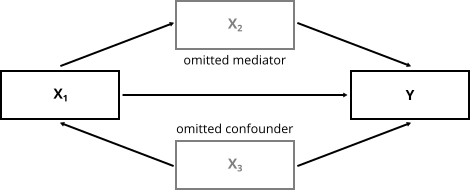
\includegraphics[width=0.95\textwidth]{images/kausal/ohne-randomisierung.png}
    \caption{Beziehung ohne Randomisierung}
    \label{img:rando-ohne}
  \end{subfigure}
  \begin{subfigure}[b]{0.47\textwidth}
    \centering
    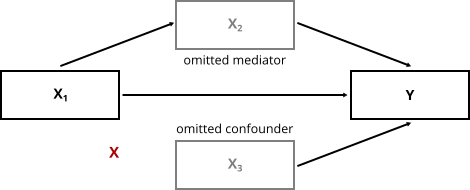
\includegraphics[width=0.95\textwidth]{images/kausal/mit-randomisierung.png}
    \caption{Beziehung mit Randomisierung}
    \label{img:rando-mit}
  \end{subfigure}
  \caption{Beziehung der Intervention $X_1$ zum Kriterium $Y$, mit \emph{omitted mediator} $X_2$ und \emph{omitted confounder} $X_3$, während der Durchführung der Intervention.}
  \label{img:rando}
\end{figure}

Auf Grund der Randomisierung haben die nicht-betrachteten Variablen (omitted variables) während der Intervention keinen Einfluss auf die betrachtete Variable. Umgekehrt bleibt ein Einfluss jedoch bestehen. Die betrachtete Variable kann weiterhin die nicht-betrachteten Variablen beeinflussen. Mit der Randomisierung wird also \emph{nur} die \emph{Konfundierung} ausgeschlossen, nicht aber die \emph{Mediation}. Der Sachverhalte ist in Abbildung~\ref{img:rando} dargestellt.

Falls die Kovarianz zwischen $X_1$ und $X_k$ nach dem Test Null ist $Cov(X_1,X_k) = 0$, kann $X_k$ ein (1a) Confounder (der jedoch keinen Einfluss hatte) sein oder $X_1$ und $X_k$ sind (1b) generell voneinander unabhängig. Falls nach dem Test $Cov(X_1,X_k) \neq 0$, ist $X_k$ ein (2a) Mediator oder es liegt eine (2b) Feedbackbeziehung vor.

Wichtig ist also: Randomisierung stellt Pseudoisolation zwischen betrachteter Variable und omitted confounders her, nicht jedoch zwischen betrachteter Variable und omitted mediators!

\paragraph*{Interpretation bei Randomisierung}

Der Steigungskoeffizient $\gamma_{11}$ ist der \textbf{erwartete totale kausale Effekte} von $X_1$ auf $Y_1$, wenn folgende Bedingungen zutreffen:

\begin{compactitem}
\item Zufällige Zuordnung der Personen in die Interventionsstufen $X_1$
\item Gerichteter Zusammenhang von $X_1$ nach $Y_1$
\item Der Steigungskoeffizient $\gamma_{11}$ ist signifikant
\end{compactitem}

\subsubsection*{Begriffe}

\fbox{\begin{minipage}{\textwidth}
Kriterien für kausale Informationen, Isolation, Kausalität bei Isolation, Ursache, Wirkung, Bedeutung des Fehlerterms, Ursache einer Abweichung, Gründe fehlender Isolation, Argumente für Kausalität bei fehlender Isolation, Pseudoisolation, omitted variables, hinreichendes Kriterium für Unkorreliertheit, omitted confounder, omitted mediator, Kausalität bei Pseudoisolation, Direkter kausaler Effekt, Randomisierung, Bedingung für Pseudoisolation, Einflüsse nicht-isolierter Variablen, Ausschluss von Konfundierung/Mediation?
\end{minipage}}


\end{document}



